\chapter{Pruning of the non-impactful nuisance parameters}
\label{chap:Appendix:AdditionalResults}
This appendix complements the fit results presented through Section~\ref{sec:ChaptH:Fit}
presenting the pruning plots for both \dileptau sub-channels.
%For the two channels, the pruning plots are pres. %Additionally, the signal strengths 
%and normalisation factors are shown for each step of the fit procedure. 


%%%%%%%%%%%%%%%%%%%
%                   Asimov OS                 %
%%%%%%%%%%%%%%%%%%%
\section{Asimov fit in the \dilepOStau channel}
\label{sec:Appendix:AdditionalResults:OS:Asimov}
Complementing Section~\ref{sec:ChaptH:Fit:ASIMOV:OS}, in this appendix
the pruning of the non-impactful NPs is presented. %in Section~\ref{sec:Appendix:AdditionalResults:OS:Asimov:Pruning}.
%The plots with the sensitivity to the $\mu_{\tHq}^{\dilepOStau}$ as well as to the $k_{\ttbar}$ and $k_{\Zjets}$  
%are shown in Section~\ref{sec:Appendix:AdditionalResults:OS:Asimov:NormFactors}.
%%%%%%%%%%%%%%%%%%%
%           Asimov OS  :: Pruning         %
%%%%%%%%%%%%%%%%%%%
%\subsection{Pruning of NPs in the \dilepOStau Asimov fit}
%\label{sec:Appendix:AdditionalResults:OS:Asimov:Pruning}
The process of removing certain NPs that have negligible impact on the
 profile likelihood fit is shown in this section. 
For all present NPs is evaluated whether to keep the parameter, to drop
its normalisation impact, to drop its shape impact or to completely drop the
NP. The shape contribution is evaluated by observing the  the maximum difference 
in bin entries between the nominal and the varied distribution, under the same 
normalisation. Regarding the normalisation contribution, it is evaluated by
integrating the nominal and varied distribution and measuring the differences.  

The pruning is shown first for the instrumental NPs in Figure~\ref{fig:Appendix:AdditionalResults:OS:Asimov:Pruning:instrumental_general}.
Here it can be seen that most of the NPs are completely pruned. 
%For the pile-up rewriting and the luminosity only the normalisation is kept in most of cases. 
Figure~\ref{fig:Appendix:AdditionalResults:OS:Asimov:Pruning:instrumental_FTAG} shows that  almost 
all the NPs dedicated to flavour tagging are fully dropped. The JES effective NPs are doped as well but this
is not the case for the JER.
The pruning of the theory-related NPs is presented in 
Figures~\ref{fig:Appendix:AdditionalResults:OS:Asimov:Pruning:Theory},~\ref{fig:Appendix:AdditionalResults:OS:Asimov:Pruning:tHqPDF}  and~\ref{fig:Appendix:AdditionalResults:OS:Asimov:Pruning:ttZPDF}. The PDF uncertainties for \ttH, \ttbar and \ttW are completely dropped. While the PDFs of the diboson and, especially, the \tHq production play an important role.


\begin{comment}
In the SR and CR(\ttbar) the \tHq PDF NPs are kept in most of cases either in shape or normalisation,
this is due to the density of \tHq events in these two regions. Meanwhile, for the CR(\Zjets) this is not
the case where either shape or the entire NP is dropped, as
Figure~\ref{fig:Appendix:AdditionalResults:OS:Asimov:Pruning:tHqPDF} illustrates.

Regarding the modelling, as Figure~\ref{fig:Appendix:AdditionalResults:OS:Asimov:Pruning:ttWPDF}
shows, the normalisation of NPs of the PDFs of the \ttW process are kept in the SR and
the CR(\ttbar) but both normalisation and shape are impactful in the CR(\Zjets). For \tZq PDFs,
Figure~\ref{fig:Appendix:AdditionalResults:OS:Asimov:Pruning:tZqPDF} manifests how
the related NPs are mostly dropped. The shape of the NPs for the PDFs of the \ttH process 
is dropped in all cases as Figure~\ref{fig:Appendix:AdditionalResults:OS:Asimov:Pruning:ttHPDF}
exhibits. With \ttZ PDFs, in Figure~\ref{fig:Appendix:AdditionalResults:OS:Asimov:Pruning:ttZPDF},
there is a similar behaviour as for \tZq.
For \ttbar, the most important background this channel, all except one NPs related to its PDFs are dropped as
Figure~\ref{fig:Appendix:AdditionalResults:OS:Asimov:Pruning:ttbarPDF} shows. Finally, for the
diboson PDFs, the shape of its NPs is dropped most of times (see 
Figure~\ref{fig:Appendix:AdditionalResults:OS:Asimov:Pruning:DibosonPDF}).
\end{comment}


\begin{figure}[h]
  \centering
  \includegraphics[width=.75\linewidth]{Chapter5_tHq/NPs/OS_new/OS_ASIMOV/Pruning_INSTRUMENTAL}	
   \caption{Pruning of non-impactful instrumental NPs in the Asimov fit of the \dilepOStau channel. Grey NPs are 
   not present and green ones are kept. Red combinations are completely dropped. For orange NPs only the shape 
   component is kept, while for yellow ones only the normalisation is kept. Additionally, the list of NPs is split by regions.}
  \label{fig:Appendix:AdditionalResults:OS:Asimov:Pruning:instrumental_general}
\end{figure}


\begin{figure}[h]
\begin{subfigure}{0.45\textwidth}
  \centering
  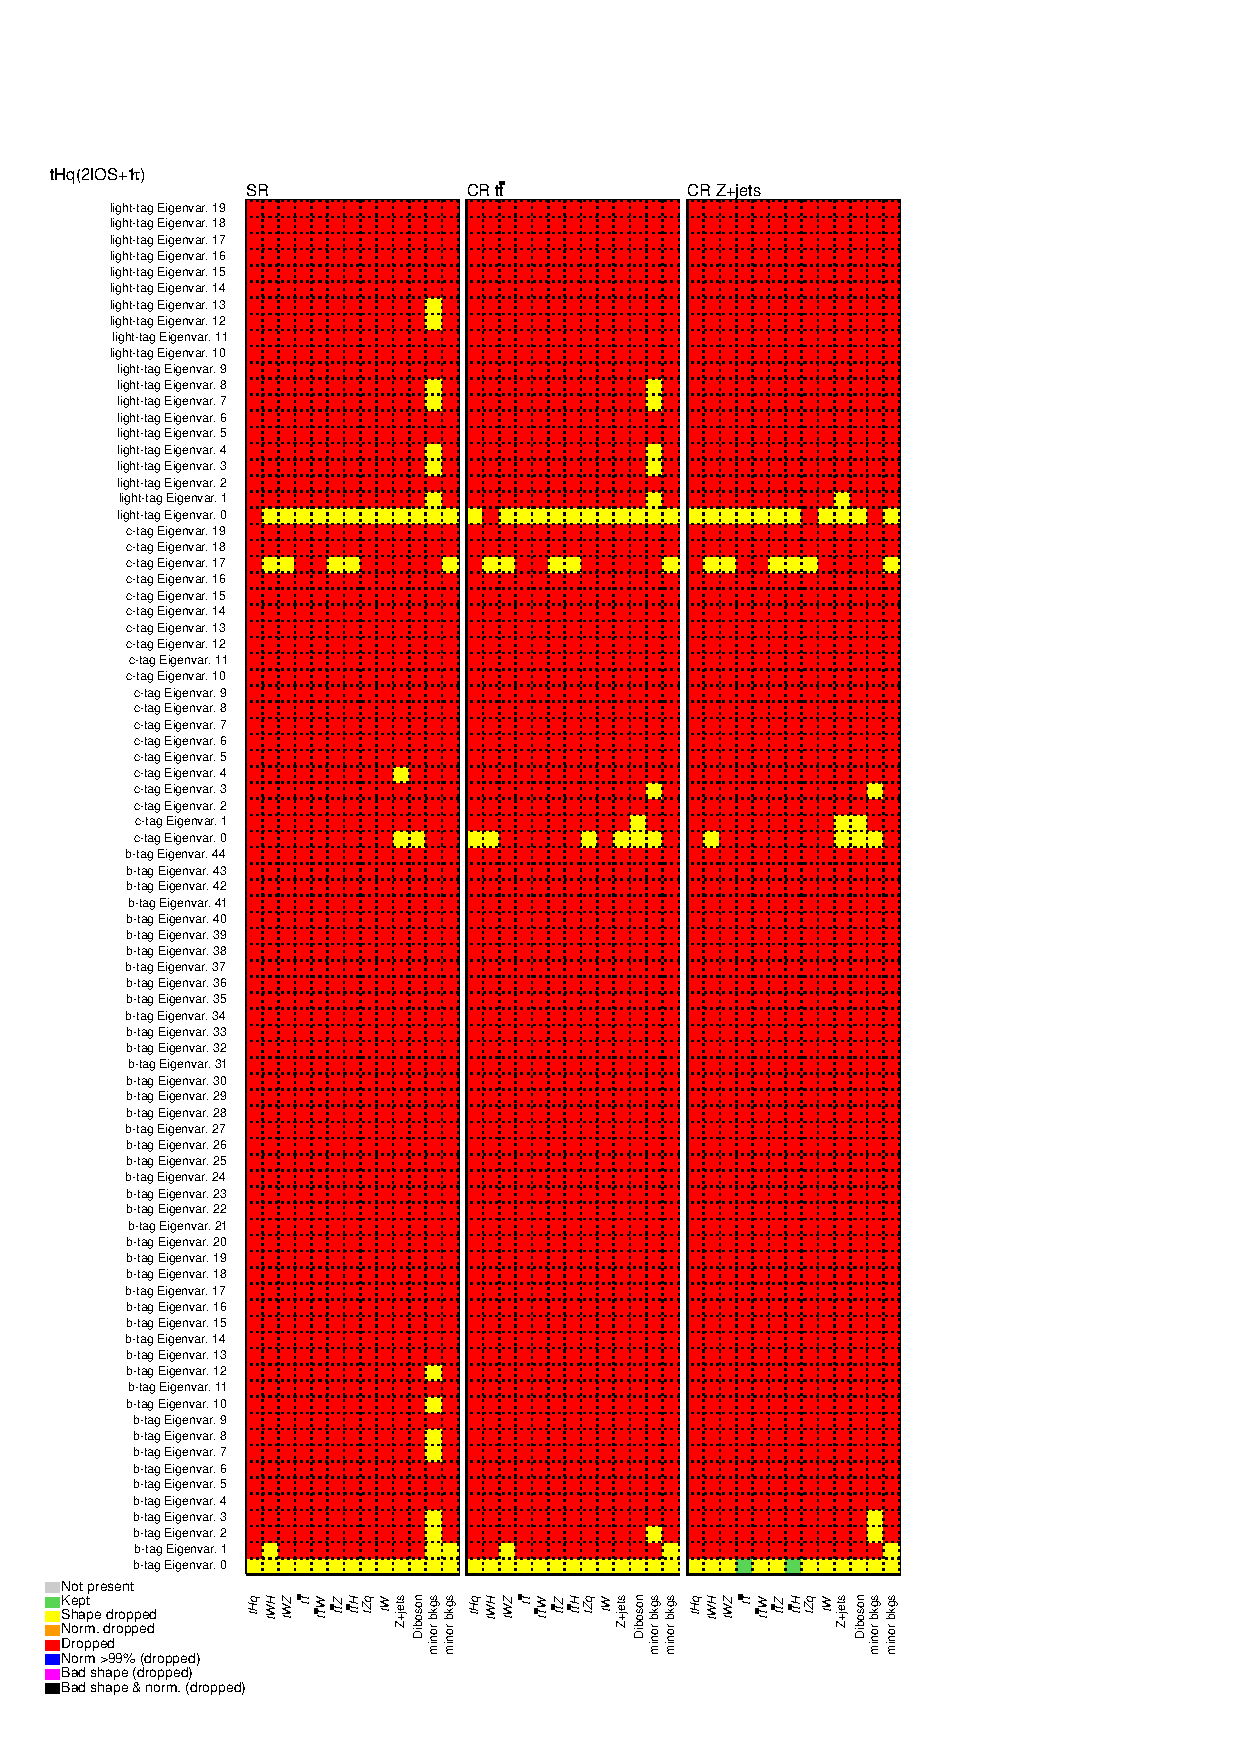
\includegraphics[width=.95\linewidth]{Chapter5_tHq/NPs/OS_new/OS_ASIMOV/Pruning_FTAG}
  \caption{}
\end{subfigure}
\hfill 
\begin{subfigure}{0.45\textwidth}
  \includegraphics[width=.95\linewidth]{Chapter5_tHq/NPs/OS_new/OS_ASIMOV/Pruning_JES}
  \caption{}
  \includegraphics[width=.95\linewidth]{Chapter5_tHq/NPs/OS_new/OS_ASIMOV/Pruning_JER}
  \caption{}
\end{subfigure}
   \caption{Pruning of non-impactful (a) flavour-tagging, (b) JES and (c) JER NPs in the Asimov fit of the \dilepOStau channel.  Grey NPs are 
   not present and green ones are kept. Red combinations are completely dropped. For orange NPs only the shape 
   component is kept, while for yellow ones only the normalisation is kept. Additionally, the list of NPs is split by regions.}
  \label{fig:Appendix:AdditionalResults:OS:Asimov:Pruning:instrumental_FTAG}
\end{figure}


\begin{figure}[h]
  \centering
  \begin{subfigure}{0.45\textwidth}
      	\includegraphics[width=.95\linewidth]{Chapter5_tHq/NPs/OS_new/OS_ASIMOV/Pruning_theory}
	\caption{}
  \end{subfigure}
  \hfill
  \begin{subfigure}{0.45\textwidth}
 	\includegraphics[width=.68\linewidth]{Chapter5_tHq/NPs/OS_new/OS_ASIMOV/Pruning_PDF_ttH}
	\caption{}
  	\includegraphics[width=.68\linewidth]{Chapter5_tHq/NPs/OS_new/OS_ASIMOV/Pruning_PDF_ttbar}  
	\caption{}
  \end{subfigure}
   \caption{Pruning of non-impactful (a) modelling NPs as well as the (b) \ttH and (c) \ttbar PDF NPs in the Asimov fit of the \dilepOStau channel. 
   The modelling NPs due to PDFs are not included in this figure. Grey NPs are 
   not present and green ones are kept. Red combinations are completely dropped. For orange NPs only the shape 
   component is kept, while for yellow ones only the normalisation is kept. Additionally, the list of NPs is split by regions.}
  \label{fig:Appendix:AdditionalResults:OS:Asimov:Pruning:Theory}
\end{figure}

\begin{figure}[h]
  \centering
  \begin{subfigure}{0.3\textwidth}
  \includegraphics[width=\linewidth]{Chapter5_tHq/NPs/OS_new/OS_ASIMOV/Pruning_PDF_tHq}
	\caption{}
  \end{subfigure}
  \begin{subfigure}{0.3\textwidth}
    \includegraphics[width=\linewidth]{Chapter5_tHq/NPs/OS_new/OS_ASIMOV/Pruning_PDF_ttW}
  	\caption{}
  \end{subfigure}
  \begin{subfigure}{0.3\textwidth}
  \includegraphics[width=\linewidth]{Chapter5_tHq/NPs/OS_new/OS_ASIMOV/Pruning_PDF_tZq}
  \caption{}
  \end{subfigure}
   \caption{Pruning of non-impactful (a) \tHq, (b) \ttW and (c) \tZq PDF NPs in the Asimov fit of the \dilepOStau channel. Grey NPs are 
   not present and green ones are kept. Red combinations are completely dropped. For orange NPs only the shape 
   component is kept, while for yellow ones only the normalisation is kept. Additionally, the list of NPs is split by regions.}
  \label{fig:Appendix:AdditionalResults:OS:Asimov:Pruning:tHqPDF}
\end{figure}


\begin{figure}[h]
  \centering
  \begin{subfigure}{0.42\textwidth}
  \includegraphics[width=\linewidth]{Chapter5_tHq/NPs/OS_new/OS_ASIMOV/Pruning_PDF_ttZ} 
  \caption{}
  \end{subfigure}
  \begin{subfigure}{0.42\textwidth}
  \includegraphics[width=\linewidth]{Chapter5_tHq/NPs/OS_new/OS_ASIMOV/Pruning_PDF_VV}
  \caption{}
  \end{subfigure}
   \caption{Pruning of non-impactful (a) \ttZ and (b) diboson PDF NPs in the Asimov fit of the \dilepOStau channel. Grey NPs are 
   not present and green ones are kept. Red combinations are completely dropped. For orange NPs only the shape 
   component is kept, while for yellow ones only the normalisation is kept. Additionally, the list of NPs is split by regions.}
  \label{fig:Appendix:AdditionalResults:OS:Asimov:Pruning:ttZPDF}
\end{figure}




\FloatBarrier

\begin{comment}
%%%%%%%%%%%%%%%%%%%%%%
%           Asimov OS  :: NormFactors          %
%%%%%%%%%%%%%%%%%%%%%%
\subsection{Normalisation factors in the \dilepOStau Asimov fit}
\label{sec:Appendix:AdditionalResults:OS:Asimov:NormFactors}

The Figure~\ref{fig:Appendix:AdditionalResults:OS:Asimov:NormFactors} 
represents graphically the results given in Equations~\ref{eq:ChaptH:ASIMOV:OS:POIs:mu},
\ref{eq:ChaptH:ASIMOV:OS:POIs:ktt}
and~\ref{eq:ChaptH:ASIMOV:OS:POIs:kzj} of Section~\ref{sec:ChaptH:Fit:ASIMOV:OS:results}.
Observe that the uncertainties are symmetrical. 


\begin{figure}[h]
\centering
\begin{subfigure}{.5\textwidth}
  \centering
  %\includegraphics[width=.95\linewidth]{Chapter5_tHq/NPs/OS/Asimov_NormFactors_statOnly}
  \includegraphics[width=.95\linewidth]{Chapter5_tHq/NPs/OS_new/OS_ASIMOV/NormFactors_statOnly}
  \caption{Using only the statistical uncertainties.}
\end{subfigure}%
\begin{subfigure}{0.5\textwidth}
  \centering
  %\includegraphics[width=.95\linewidth]{Chapter5_tHq/NPs/OS/Asimov_NormFactors}
  \includegraphics[width=.95\linewidth]{Chapter5_tHq/NPs/OS_new/OS_ASIMOV/NormFactors}
  \caption{Considering all uncertainties.}
\end{subfigure}
\caption{Sensitivity to the signal strength and normalisation factors calculated the Asimov fit of the \dilepOStau channel.}
\label{fig:Appendix:AdditionalResults:OS:Asimov:NormFactors}
\end{figure}



\FloatBarrier
%%%%%%%%%%%%%%%%%%
%          CRONLY BONLY OS        %
%%%%%%%%%%%%%%%%%%
\section{CR-only--background-only fit in the \dilepOStau channel}
\label{sec:Appendix:AdditionalResults:OS:CRBONLY}


\FloatBarrier
%%%%%%%%%%%%%%%%%%%%%%%%%%%
%           CRONLY BONLY OS  :: NormFactors          %
%%%%%%%%%%%%%%%%%%%%%%%%%%%
\subsection{Normalisation factors  in the \dilepOStau CR-only--background-only fit}
\label{sec:Appendix:AdditionalResults:OS:CRBONLY:NormFactors}

\begin{figure}[h]
\centering
\begin{subfigure}{.5\textwidth}
  \centering
  %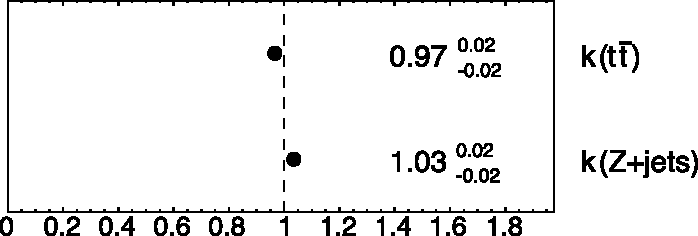
\includegraphics[width=.95\linewidth]{Chapter5_tHq/NPs/OS/CRBONLY_NormFactors_statOnly}
  \includegraphics[width=.95\linewidth]{Chapter5_tHq/NPs//OS_new/OS_BONLYCRONLY/NormFactors_statOnly}
  \caption{Using only the statistical uncertainties.}
\end{subfigure}%
\begin{subfigure}{0.5\textwidth}
  \centering
  %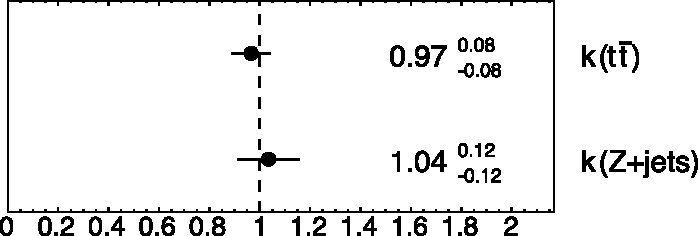
\includegraphics[width=.95\linewidth]{Chapter5_tHq/NPs/OS/CRBONLY_NormFactors}
  \includegraphics[width=.95\linewidth]{Chapter5_tHq/NPs//OS_new/OS_BONLYCRONLY/NormFactors}
  \caption{Considering all uncertainties.}
\end{subfigure}
\caption{Normalisation factors in the CR-only--background-only fit of the \dilepOStau channel.
These results are obtained with (a) the fit considering only the statistical uncertainty and (b) the
considering all uncertainty sources.}
\label{fig:Appendix:AdditionalResults:OS:CRBONLY:NormFactors}
\end{figure}



%%%%%%%%%%%%%%%%%%
%              Full data fit OS              %
%%%%%%%%%%%%%%%%%%
\section{Full-data-unblinded fit in the \dilepOStau channel}
\label{sec:Appendix:AdditionalResults:OS:Unblinded}

%\subsection{Pruning}
%\label{sec:Appendix:AdditionalResults:OS:Unblinded:Pruning}



\FloatBarrier

%%%%%%%%%%%%%%%%%%%%%%%%%%
%              Full data fit OS  :: NormFactors            %
%%%%%%%%%%%%%%%%%%%%%%%%%
\subsection{Normalisation factors in the \dilepOStau full-data-unblinded fit}
\label{sec:Appendix:AdditionalResults:OS:Unblinded:NormFactors}

The Figure~\ref{fig:Appendix:AdditionalResults:OS:Unblinded:NormFactors} 
represents graphically the results given in Equations~\ref{eq:ChaptH:FinalFit:OS:mu},
\ref{eq:ChaptH:FinalFit:OS:ktt}
and~\ref{eq:ChaptH:FinalFit:OS:zjets} of Section~\ref{sec:ChaptH:Fit:FullFit:OS:results}.
Observe that the uncertainties are symmetrical. 


\begin{figure}[h]
\centering
\begin{subfigure}{.5\textwidth}
  \centering
  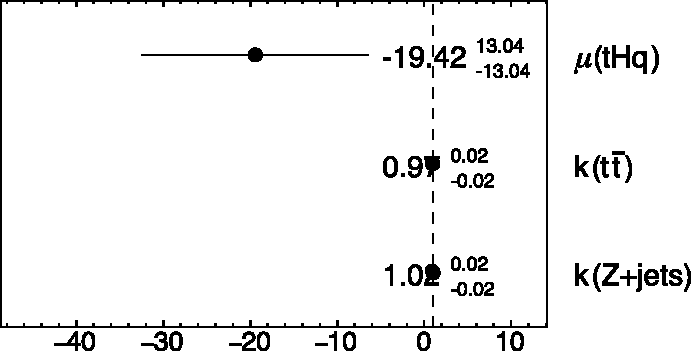
\includegraphics[width=.95\linewidth]{Chapter5_tHq/NPs/OS/Unblinded_NormFactors_statOnly}
  \caption{Using only the statistical uncertainties.}
\end{subfigure}%
\begin{subfigure}{0.5\textwidth}
  \centering
  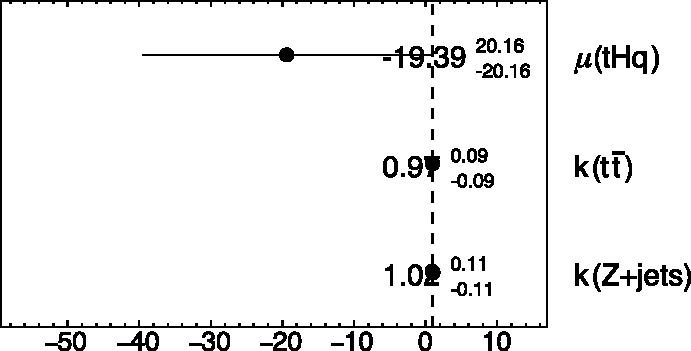
\includegraphics[width=.95\linewidth]{Chapter5_tHq/NPs/OS/Unblinded_NormFactors}
  \caption{Considering all uncertainties.}
\end{subfigure}
\caption{Normalisation factors in the full-data-unblinded fit of the \dilepOStau channel.
 These results are obtained with (a) the fit considering only the statistical uncertainty and (b) the
considering all uncertainty sources.}
\label{fig:Appendix:AdditionalResults:OS:Unblinded:NormFactors}
\end{figure}

\FloatBarrier
\end{comment}


%%%%%%%%%%%%
%          Asimov SS     %
%%%%%%%%%%%%
\section{Asimov fit in the \dilepSStau channel}
\label{sec:Appendix:AdditionalResults:SS:Asimov}
Complementing Section~\ref{sec:ChaptH:Fit:ASIMOV:SS}, in this appendix
the pruning of the non-impactful NPs is presented. % in Section~\ref{sec:Appendix:AdditionalResults:SS:Asimov:Pruning}.
%The plots with the sensitivity to the $\mu_{\tHq}^{\dilepSStau}$ as well as to the $k_{\ttbar,\ttX}$ normalisation factor 
%are shown in Section~\ref{sec:Appendix:AdditionalResults:SS:Asimov:NormFactors}.
%%%%%%%%%%%%%%%%%%%
%           Asimov SS  :: Pruning         %
%%%%%%%%%%%%%%%%%%%
%\subsection{Pruning}
%\label{sec:Appendix:AdditionalResults:SS:Asimov:Pruning}
The pruning of the experimental NPs in the \dilepSStau channel 
is presented in Figure~\ref{fig:Appendix:AdditionalResults:SS:Asimov:Pruning:instrumental_general}.
For the theory-related NPs is presented these results are shown in
Figures~\ref{fig:Appendix:AdditionalResults:SS:Asimov:Pruning:Theory},~\ref{fig:Appendix:AdditionalResults:SS:Asimov:Pruning:tHqPDF} 
and~\ref{fig:Appendix:AdditionalResults:SS:Asimov:Pruning:ttZPDF}. Note that the PDF uncertainties for \ttH, \ttbar and \ttW are completely dropped.

\begin{figure}[h]
  \centering
  \includegraphics[height=0.6\textheight]{Chapter5_tHq/NPs/SS_new/SS_ASIMOV/Pruning_INSTRUMENTAL}
   \caption{Pruning of non-impactful instrumental NPs in the Asimov fit of the \dilepSStau channel. Grey NPs are 
   not present and green ones are kept. Red combinations are completely dropped. For orange NPs only the shape 
   component is kept, while for yellow ones only the normalisation is kept. Additionally, the list of NPs is split by regions.}
  \label{fig:Appendix:AdditionalResults:SS:Asimov:Pruning:instrumental_general}
\end{figure}





\begin{figure}[h]
\begin{subfigure}{0.45\textwidth}
  \centering
  %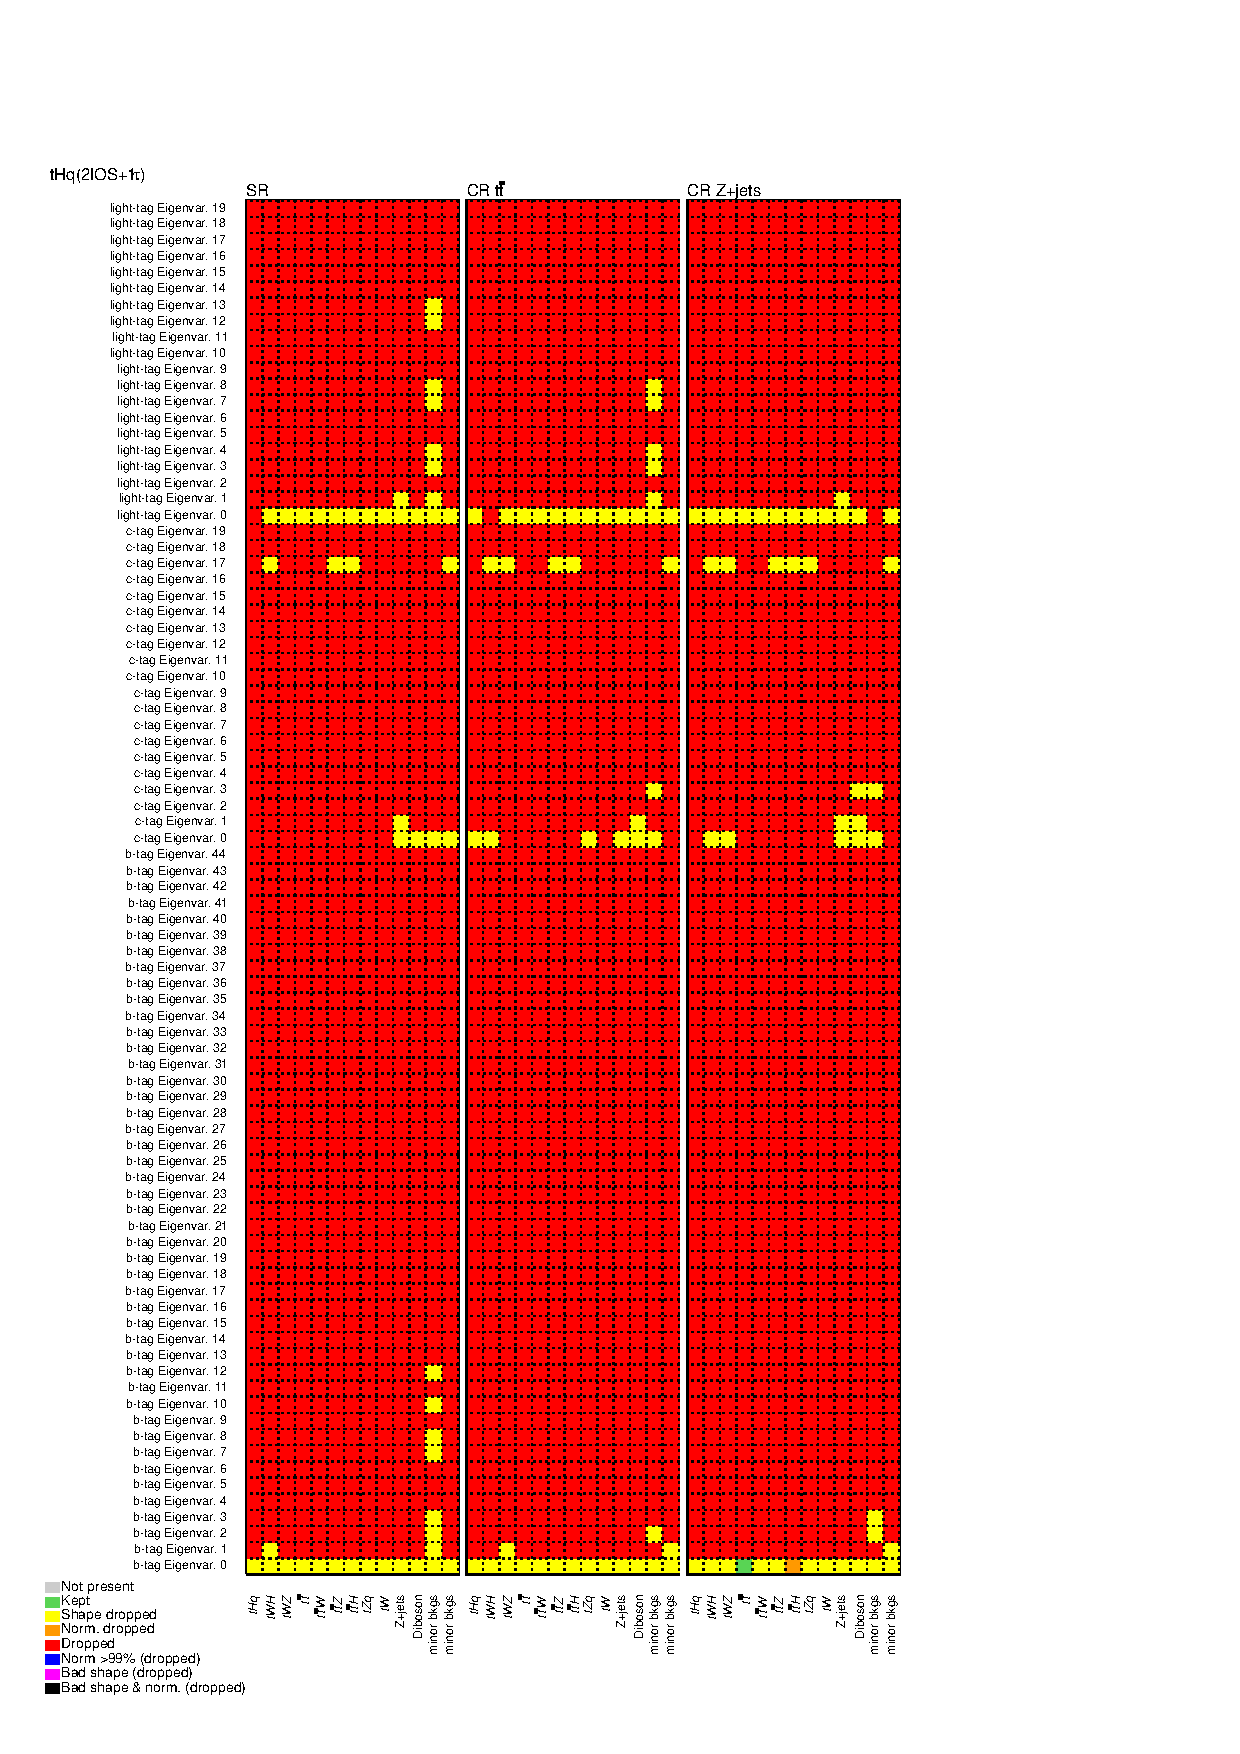
\includegraphics[height=0.9\textheight]{Chapter5_tHq/NPs/OS/Asimov_Pruning_divided_Pruning_instrumental_FTAG}
  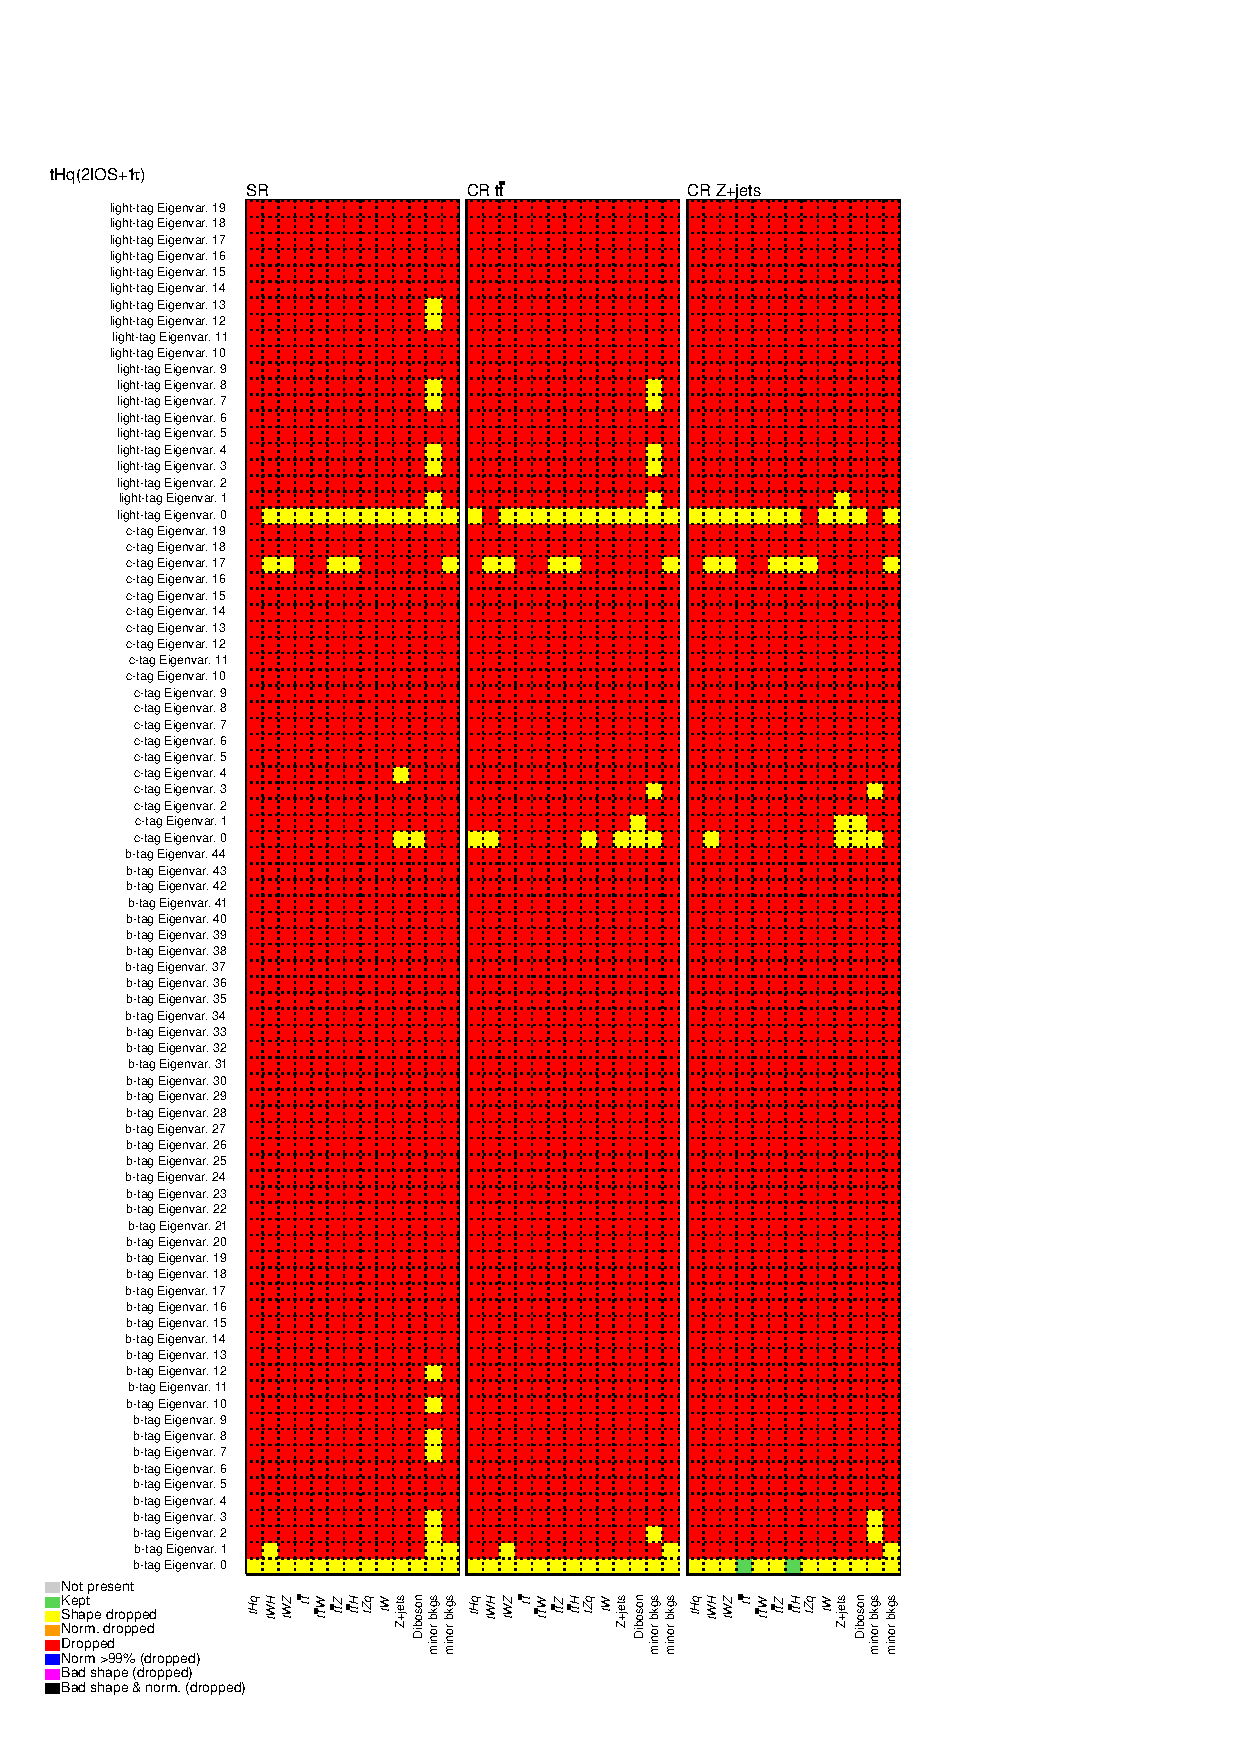
\includegraphics[width=.95\linewidth]{Chapter5_tHq/NPs/OS_new/OS_ASIMOV/Pruning_FTAG}
  \caption{}
\end{subfigure}
\hfill 
\begin{subfigure}{0.45\textwidth}
  \includegraphics[width=.95\linewidth]{Chapter5_tHq/NPs/SS_new/SS_ASIMOV/Pruning_JES}
  \caption{}
  \includegraphics[width=.95\linewidth]{Chapter5_tHq/NPs/SS_new/SS_ASIMOV/Pruning_JER}
  \caption{}
\end{subfigure}
   \caption{Pruning of non-impactful (a) flavour-tagging, (b) JES and (c) JER NPs in the Asimov fit of the \dilepSStau channel. Grey NPs are 
   not present and green ones are kept. Red combinations are completely dropped. For orange NPs only the shape 
   component is kept, while for yellow ones only the normalisation is kept. Additionally, the list of NPs is split by regions.}
  \label{fig:Appendix:AdditionalResults:SS:Asimov:Pruning:instrumental_FTAG}
\end{figure}




\begin{figure}[h]
  \centering
  \begin{subfigure}{0.45\textwidth}
      	\includegraphics[width=.95\linewidth]{Chapter5_tHq/NPs/SS_new/SS_ASIMOV/Pruning_theory}
	\caption{}
  \end{subfigure}
  \hfill
  \begin{subfigure}{0.45\textwidth}
 	\includegraphics[width=.68\linewidth]{Chapter5_tHq/NPs/SS_new/SS_ASIMOV/Pruning_PDF_ttH}
	\caption{}
  	\includegraphics[width=.68\linewidth]{Chapter5_tHq/NPs/SS_new/SS_ASIMOV/Pruning_PDF_ttbar}
	\caption{}  
  \end{subfigure}
   \caption{Pruning of non-impactful (a) modelling NPs as well as the (b) \ttH and (c) \ttbar PDF NPs in the Asimov fit of the \dilepSStau channel. 
   The modelling NPs due to PDFs are not included in this figure. Grey NPs are 
   not present and green ones are kept. Red combinations are completely dropped. For orange NPs only the shape 
   component is kept, while for yellow ones only the normalisation is kept. Additionally, the list of NPs is split by regions.}
  \label{fig:Appendix:AdditionalResults:SS:Asimov:Pruning:Theory}
\end{figure}

\begin{figure}[h]
  \centering
  %\includegraphics[height=0.9\textheight]{Chapter5_tHq/NPs/SS_new/SS_ASIMOV/Pruning_PDF_tHq}
    \begin{subfigure}{0.3\textwidth}
  \includegraphics[width=\linewidth]{Chapter5_tHq/NPs/SS_new/SS_ASIMOV/Pruning_PDF_tHq}
	\caption{}
  \end{subfigure}
  \begin{subfigure}{0.3\textwidth}
    \includegraphics[width=\linewidth]{Chapter5_tHq/NPs/SS_new/SS_ASIMOV/Pruning_PDF_ttW}
  	\caption{}
  \end{subfigure}
  \begin{subfigure}{0.3\textwidth}
  \includegraphics[width=\linewidth]{Chapter5_tHq/NPs/SS_new/SS_ASIMOV/Pruning_PDF_tZq}
  \caption{}
  \end{subfigure}
   \caption{Pruning of non-impactful (a) \tHq, (c) \ttW and (c) \tZq PDF NPs in the Asimov fit of the \dilepSStau channel. Grey NPs are 
   not present and green ones are kept. Red combinations are completely dropped. For orange NPs only the shape 
   component is kept, while for yellow ones only the normalisation is kept. Additionally, the list of NPs is split by regions.}
  \label{fig:Appendix:AdditionalResults:SS:Asimov:Pruning:tHqPDF}
\end{figure}

%\begin{figure}[h]
%  \centering
%  \includegraphics[height=0.9\textheight]{Chapter5_tHq/NPs/SS_new/SS_ASIMOV/Pruning_PDF_ttW}
%   \caption{Pruning of non-impactful \ttW PDF NPs in the Asimov fit of the \dilepSStau channel. Grey NPs are 
%   not present and green ones are kept. Red combinations are completely dropped. For orange NPs only the shape 
%   component is kept, while for yellow ones only the normalisation is kept. Additionally, the list of NPs is split by regions.}
%  \label{fig:Appendix:AdditionalResults:SS:Asimov:Pruning:ttWPDF}
%\end{figure}

%\begin{figure}[h]
%  \centering
%  \includegraphics[height=0.9\textheight]{Chapter5_tHq/NPs/SS_new/SS_ASIMOV/Pruning_PDF_tZq}
%   \caption{Pruning of non-impactful \tZq PDF NPs in the Asimov fit of the \dilepSStau channel. Grey NPs are 
%   not present and green ones are kept. Red combinations are completely dropped. For orange NPs only the shape 
%   component is kept, while for yellow ones only the normalisation is kept. Additionally, the list of NPs is split by regions.}
%  \label{fig:Appendix:AdditionalResults:SS:Asimov:Pruning:tZqPDF}
%\end{figure}


%\begin{figure}[h]
%  \centering
%  \includegraphics[width=.85\linewidth]{Chapter5_tHq/NPs/SS_new/SS_ASIMOV/Pruning_PDF_ttbar}
%   \caption{Pruning of non-impactful \ttbar PDF NPs in the Asimov fit of the \dilepSStau channel. Grey NPs are 
%   not present and green ones are kept. Red combinations are completely dropped. For orange NPs only the shape 
%   component is kept, while for yellow ones only the normalisation is kept. Additionally, the list of NPs is split by regions.}
%  \label{fig:Appendix:AdditionalResults:SS:Asimov:Pruning:ttbarPDF}
%\end{figure}


\begin{figure}[h]
  \centering
  \begin{subfigure}{0.42\textwidth}
  \includegraphics[width=\linewidth]{Chapter5_tHq/NPs/SS_new/SS_ASIMOV/Pruning_PDF_ttZ} 
  \caption{}
  \end{subfigure}
  \begin{subfigure}{0.42\textwidth}
  \includegraphics[width=\linewidth]{Chapter5_tHq/NPs/SS_new/SS_ASIMOV/Pruning_PDF_VV}
  \caption{}
  \end{subfigure}
   \caption{Pruning of non-impactful (a) \ttZ and (b) Diboson PDFs NPs in the Asimov fit of the \dilepSStau channel. Grey NPs are 
   not present and green ones are kept. Red combinations are completely dropped. For orange NPs only the shape 
   component is kept, while for yellow ones only the normalisation is kept. Additionally, the list of NPs is split by regions.}
  \label{fig:Appendix:AdditionalResults:SS:Asimov:Pruning:ttZPDF}
\end{figure}

%\begin{figure}[h]
%  \centering
%  \includegraphics[height=0.9\textheight]{Chapter5_tHq/NPs/SS_new/SS_ASIMOV/Pruning_PDF_VV}
%   \caption{Pruning of non-impactful diboson PDF NPs in the Asimov fit of the \dilepSStau channel. Grey NPs are 
%   not present and green ones are kept. Red combinations are completely dropped. For orange NPs only the shape 
%   component is kept, while for yellow ones only the normalisation is kept. Additionally, the list of NPs is split by regions.}
%  \label{fig:Appendix:AdditionalResults:SS:Asimov:Pruning:DibosonPDF}
%\end{figure}

\begin{comment}

\FloatBarrier
%%%%%%%%%%%%%%%%%%%%%
%           Asimov SS  :: NormFactors         %
%%%%%%%%%%%%%%%%%%%%%
\subsection{Normalisation factors in the \dilepSStau Asimov fit}
\label{sec:Appendix:AdditionalResults:SS:Asimov:NormFactors}

The Figure~\ref{fig:Appendix:AdditionalResults:SS:Asimov:NormFactors} 
represents graphically the results given in Equations~\ref{eq:ChaptH:Fit:ASIMOV:SS:mu}
and~\ref{eq:ChaptH:Fit:ASIMOV:SS:k} of Section~\ref{sec:ChaptH:Fit:ASIMOV:SS:results}.
Observe that the uncertainties are symmetrical. 


\begin{figure}[h]
\centering
\begin{subfigure}{.5\textwidth}
  \centering
  \includegraphics[width=.95\linewidth]{Chapter5_tHq/NPs/SS/SingleCR/Asimov_NormFactors_statOnly}
  \caption{Using only the statistical uncertainties.}
\end{subfigure}%
\begin{subfigure}{0.5\textwidth}
  \centering
  \includegraphics[width=.95\linewidth]{Chapter5_tHq/NPs/SS/SingleCR/Asimov_NormFactors}
  \caption{Considering all uncertainties.}
\end{subfigure}
\caption{Sensitivity to the signal strength and normalisation factor calculated the Asimov fit of the \dilepSStau channel.}
\label{fig:Appendix:AdditionalResults:SS:Asimov:NormFactors}
\end{figure}

\FloatBarrier

%%%%%%%%%%%%%%%%%%
%          CRONLY BONLY SS        %
%%%%%%%%%%%%%%%%%%
\section{CR-only--background-only fit in the \dilepSStau channel}
\label{sec:Appendix:AdditionalResults:SS:CRBONLY} 

%%%%%%%%%%%%%%%%%%%%%%%
%           CRONLY BONLY SS  :: Pulls          %
%%%%%%%%%%%%%%%%%%%%%%%
\subsection{Pull plots in the \dilepSStau CR-only--background-only fit}
\label{sec:Appendix:AdditionalResults:SS:CRBONLY:Pulls}

\begin{figure}[h]
  \centering
  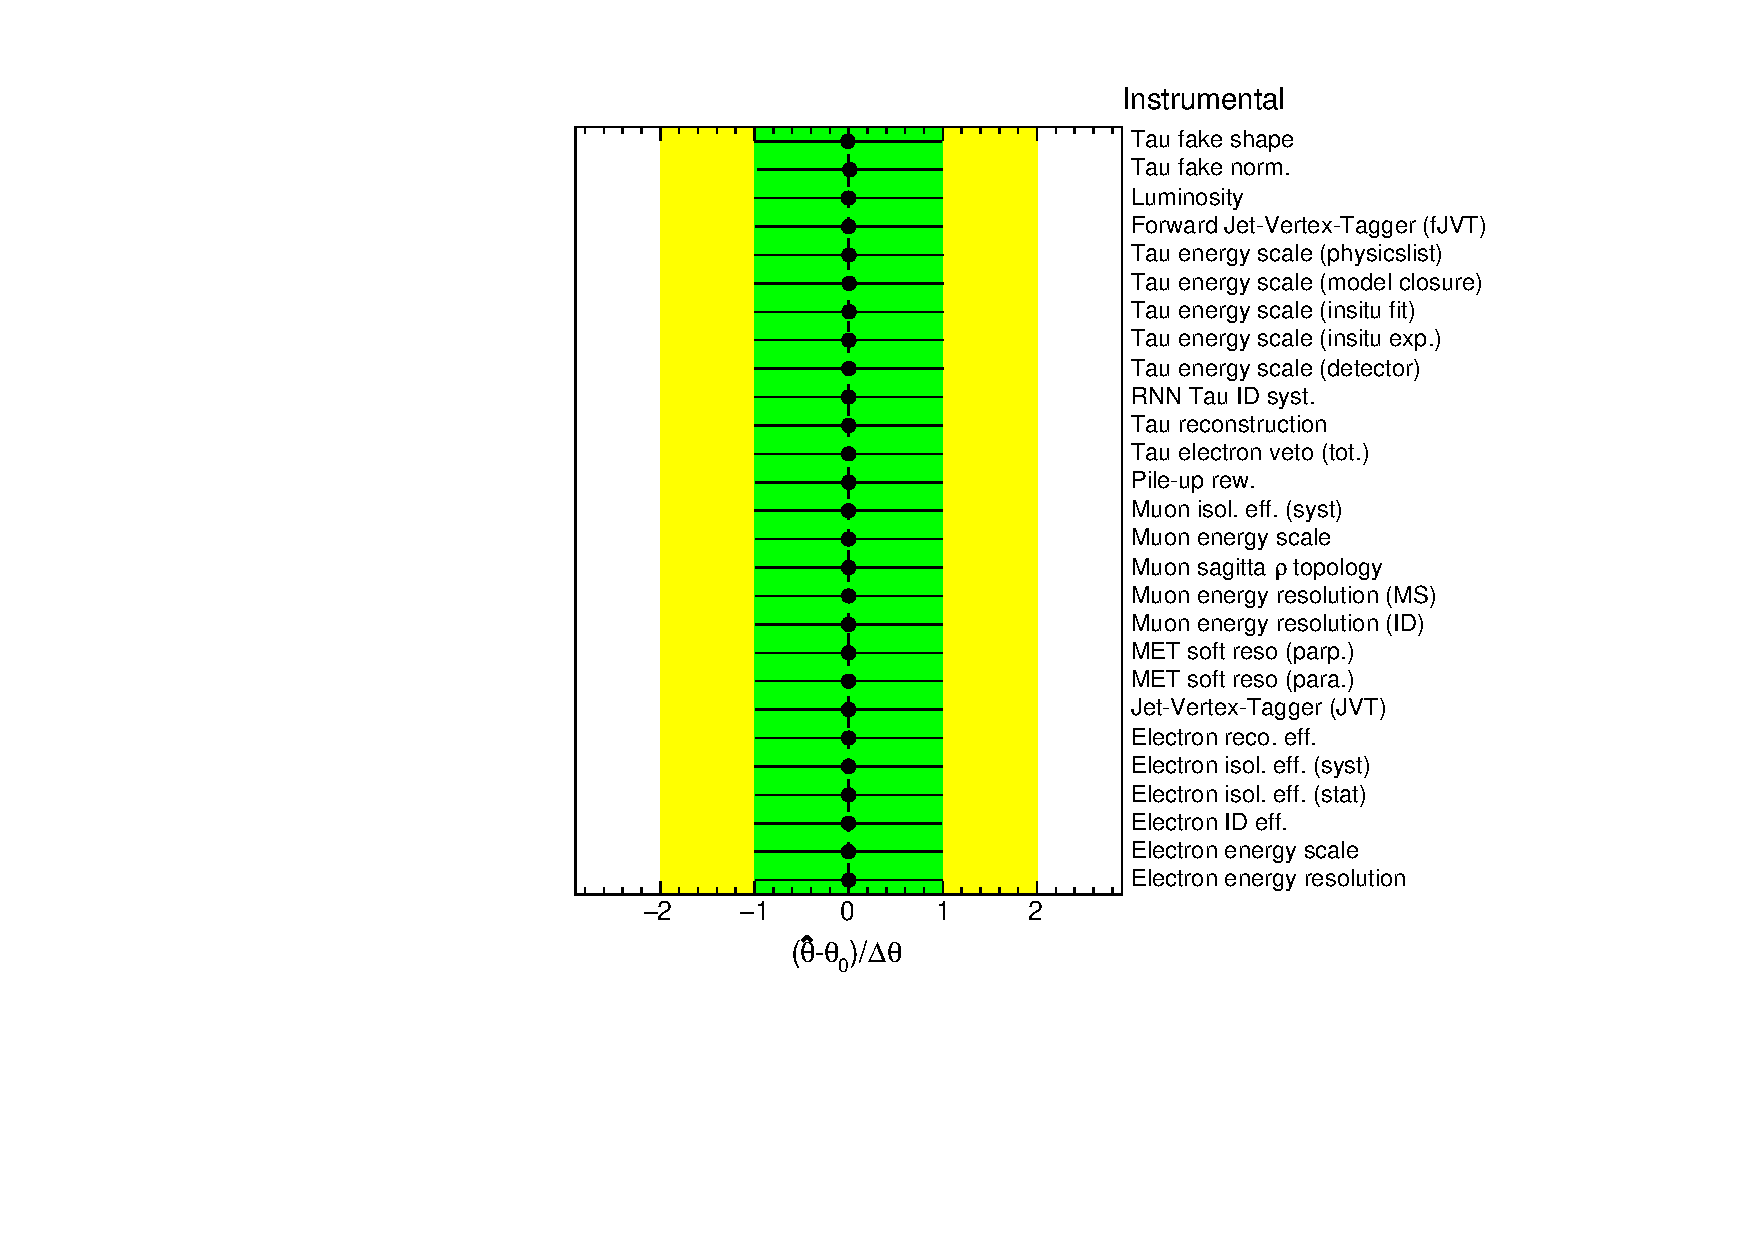
\includegraphics[width=.95\linewidth]{Chapter5_tHq/NPs/SS/SingleCR/CRBONLY_NuisPar_Instrumental}
   \caption{Constraints and pulls Constraints and pulls on the instrumental NPs in the CR-only--background-only fit of the \dilepSStau channel.
   Each NP is shown as the relative change from its nominal value.
   The green and yellow areas represent the $\pm1\sigma$ and $\pm2\sigma$ deviations from the nominal value of the NP, respectively. 
   The points represent the best-fit value for the NP and the uncertainty bars represent the post-fit uncertainty.}
  \label{fig:Appendix:AdditionalResults:SS:CRBONLY:NuisPar_Instrumental}
\end{figure}

\begin{figure}[h]
  \centering
  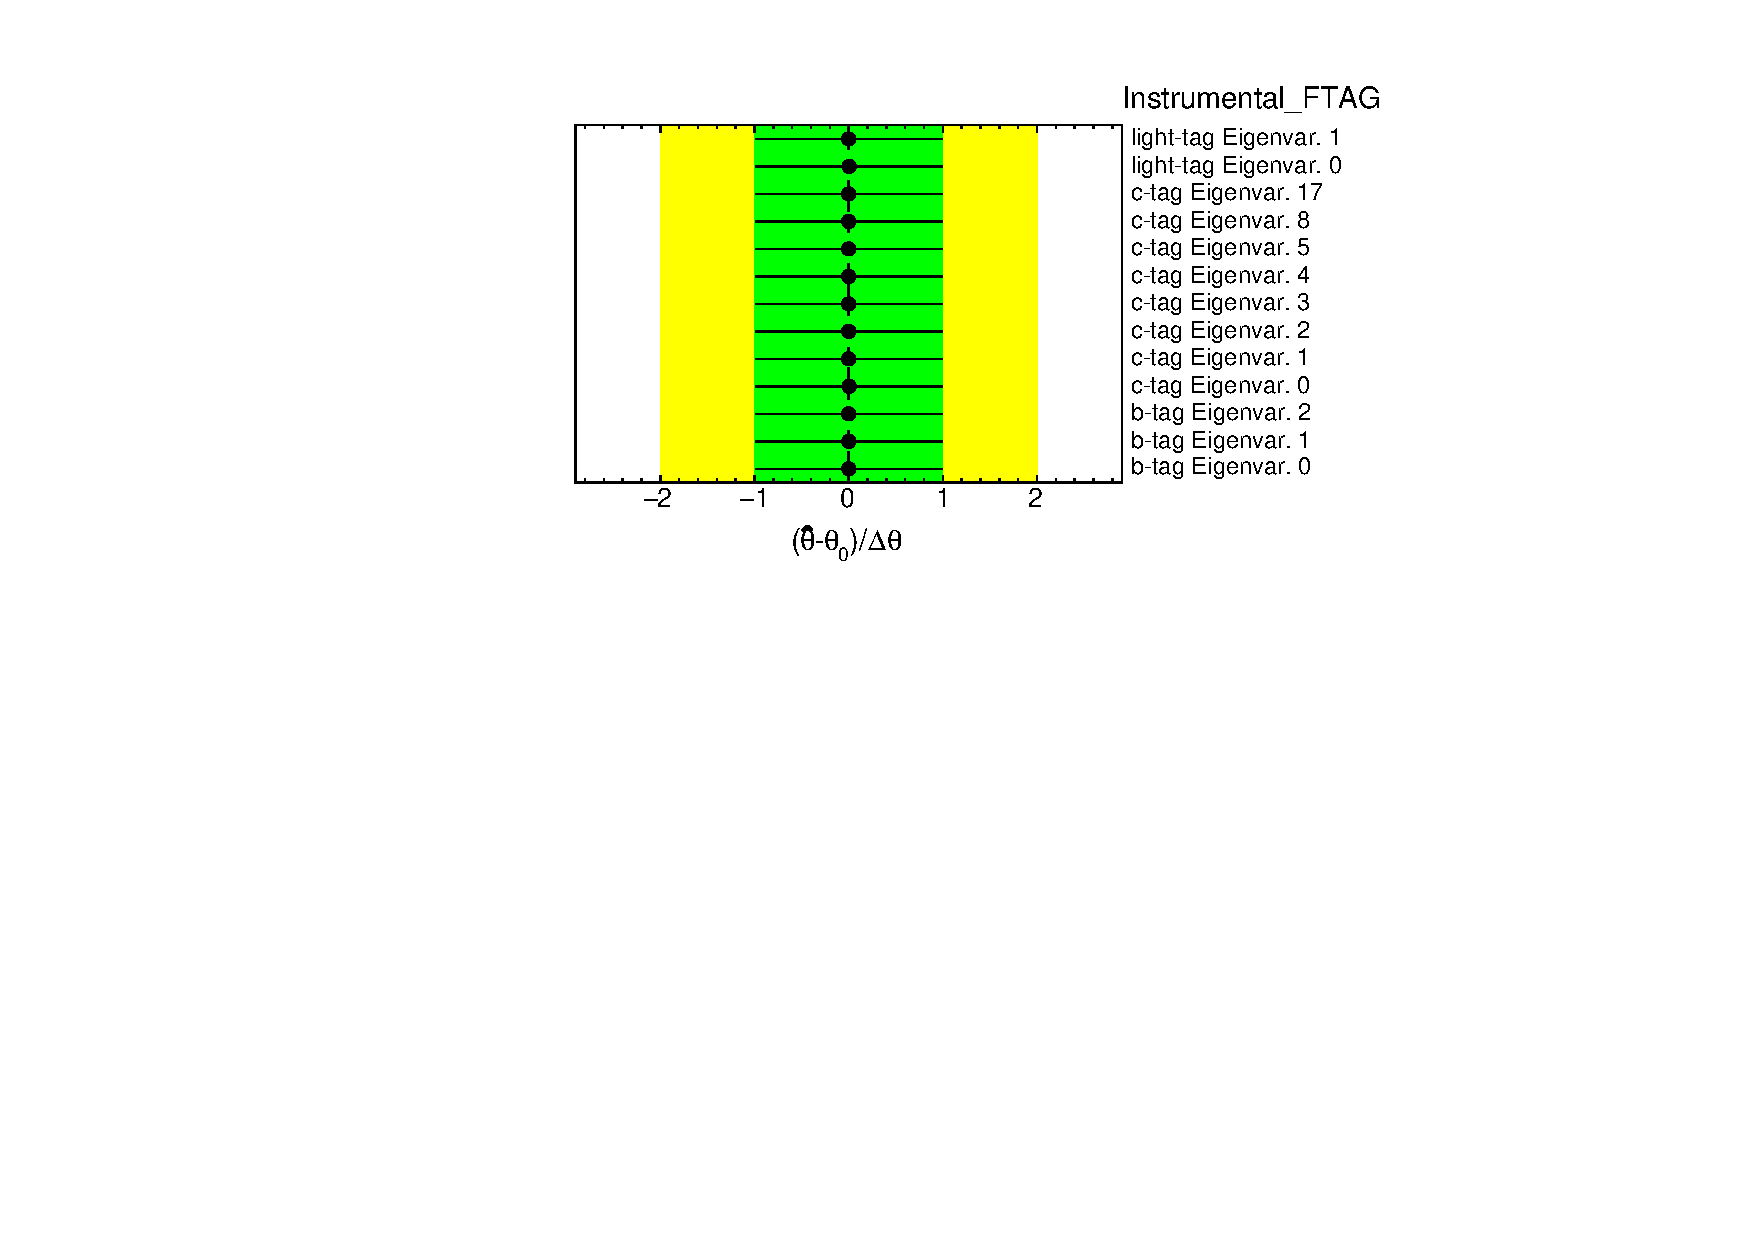
\includegraphics[width=.95\linewidth]{Chapter5_tHq/NPs/SS/SingleCR/CRBONLY_NuisPar_Instrumental_FTAG}
   \caption{Constraints and pulls on the NPs of flavour tagging in the CR-only--background-only fit of the \dilepSStau channel.
   Each NP is shown as the relative change from its nominal value.
   The green and yellow areas represent the $\pm1\sigma$ and $\pm2\sigma$ deviations from the nominal value of the NP, respectively. 
   The points represent the best-fit value for the NP and the uncertainty bars represent the post-fit uncertainty.}
  \label{fig:Appendix:AdditionalResults:SS:CRBONLY:NuisPar_Instrumental_FTAG}
\end{figure}

\begin{figure}[h]
  \centering
  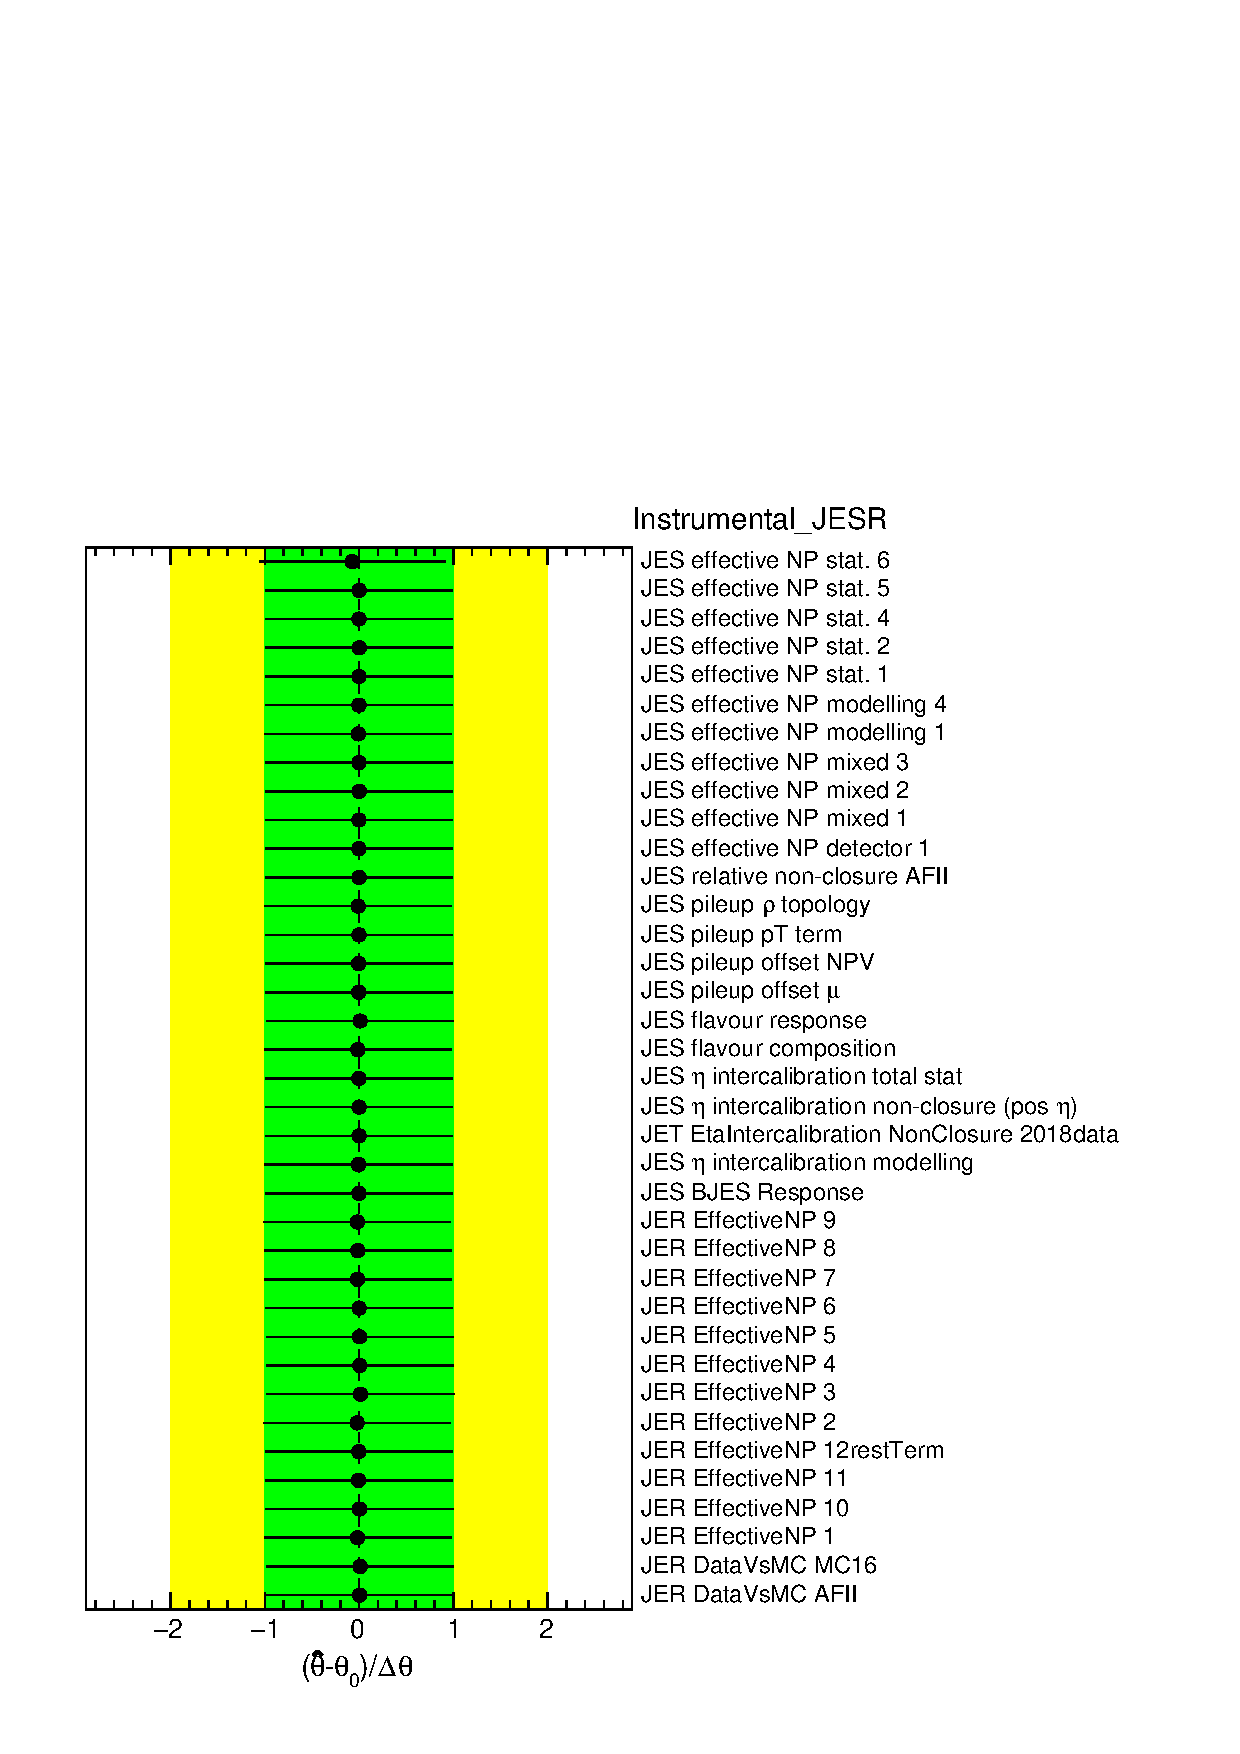
\includegraphics[width=.95\linewidth]{Chapter5_tHq/NPs/SS/SingleCR/CRBONLY_NuisPar_Instrumental_JESR}
   \caption{Constraints and pulls on the NPs of the JES and JER in the CR-only--background-only fit of the \dilepSStau channel.
   Each NP is shown as the relative change from its nominal value.
   The green and yellow areas represent the $\pm1\sigma$ and $\pm2\sigma$ deviations from the nominal value of the NP, respectively. 
   The points represent the best-fit value for the NP and the uncertainty bars represent the post-fit uncertainty.}
  \label{fig:Appendix:AdditionalResults:SS:CRBONLY:NuisPar_Instrumental_JESR}
\end{figure}


\begin{figure}[h]
  \centering
  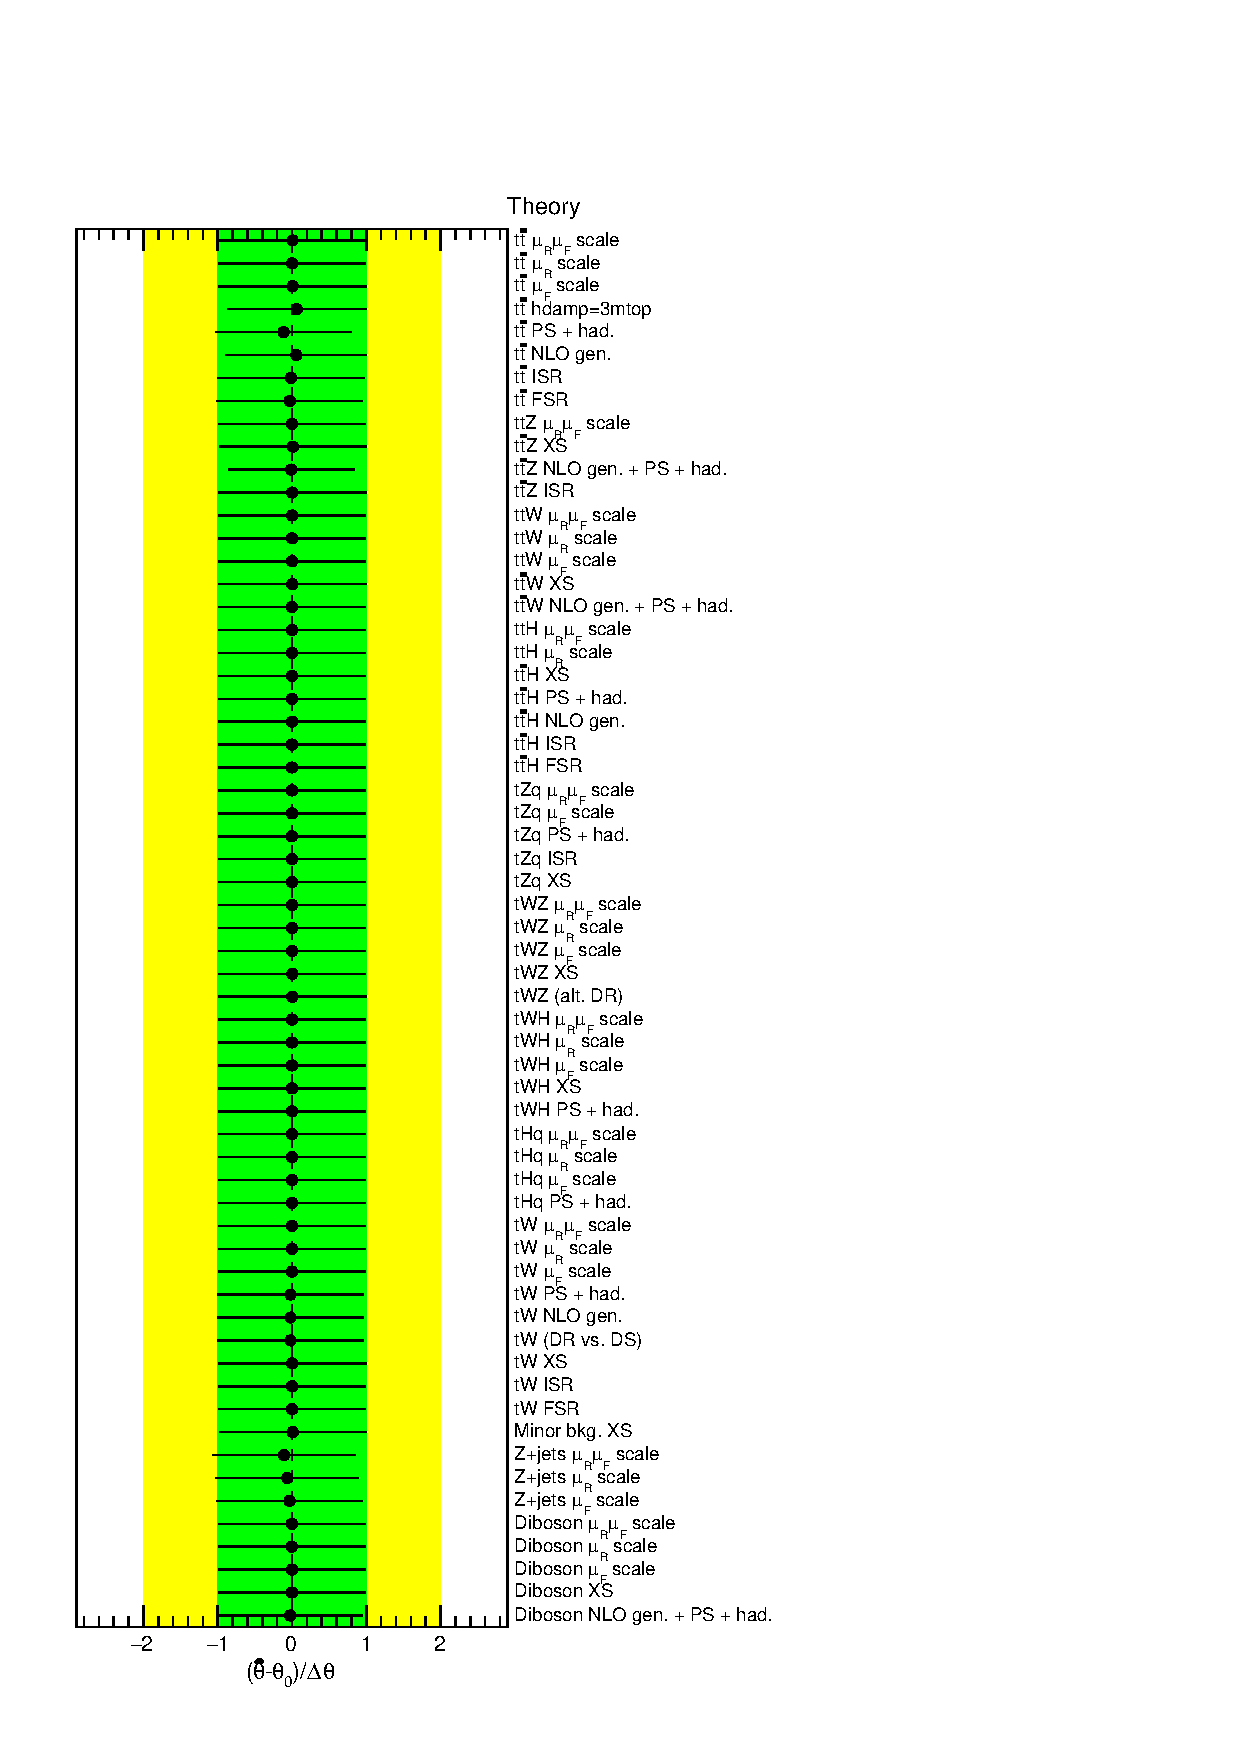
\includegraphics[width=.95\linewidth]{Chapter5_tHq/NPs/SS/SingleCR/CRBONLY_NuisPar_Theory}
   \caption{Constraints and pulls on the modelling NPs in the CR-only--background-only fit of the \dilepSStau channel.
   Each NP is shown as the relative change from its nominal value.
   The green and yellow areas represent the $\pm1\sigma$ and $\pm2\sigma$ deviations from the nominal value of the NP, respectively. 
   The points represent the best-fit value for the NP and the uncertainty bars represent the post-fit uncertainty.}
  \label{fig:Appendix:AdditionalResults:SS:CRBONLY:NuisPar_Theory}
\end{figure}

\begin{figure}[h]
  \centering
  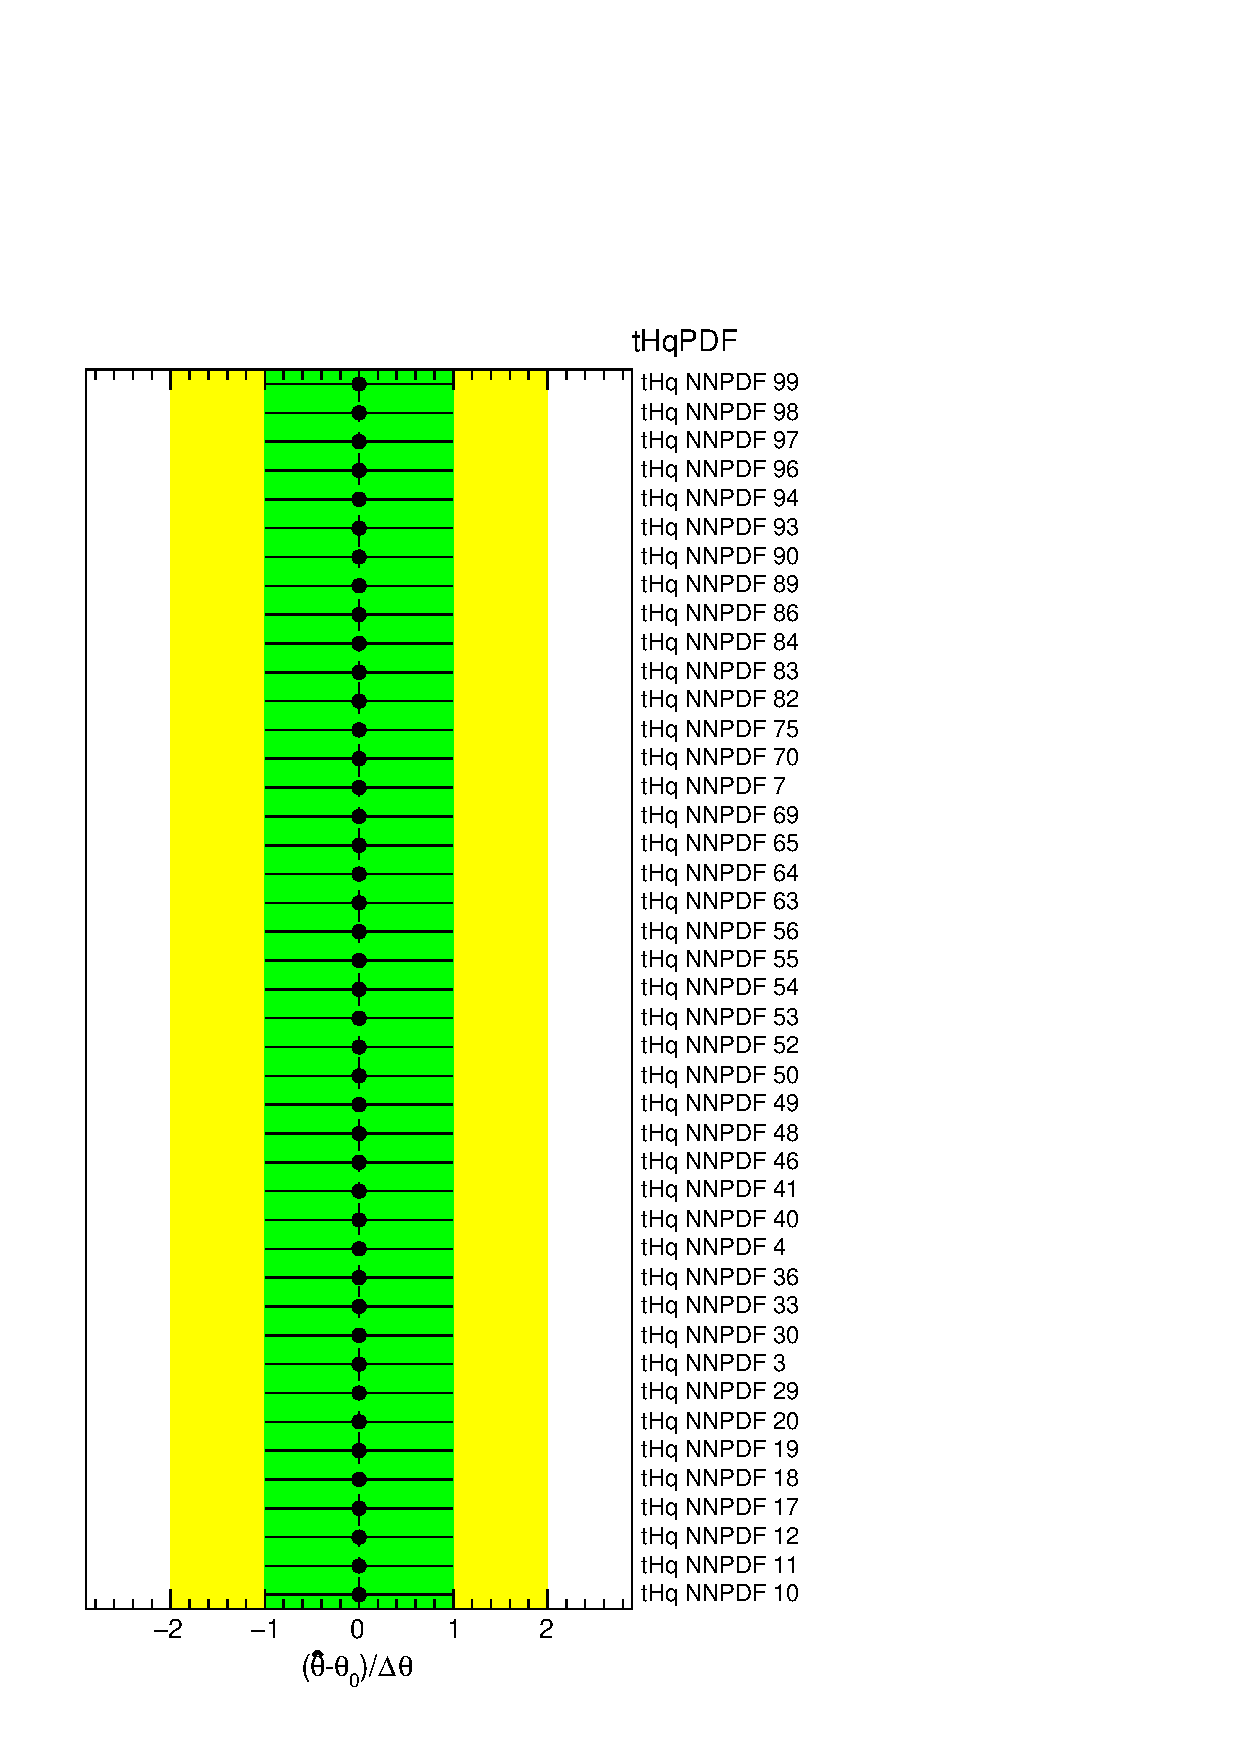
\includegraphics[height=0.9\textheight]{Chapter5_tHq/NPs/SS/SingleCR/CRBONLY_NuisPar_tHqPDF}
   \caption{Constraints and pulls on the NPs of the \tHq PDFs in the CR-only--background-only fit of the \dilepSStau channel.
   Each NP is shown as the relative change from its nominal value.
   The green and yellow areas represent the $\pm1\sigma$ and $\pm2\sigma$ deviations from the nominal value of the NP, respectively. 
   The points represent the best-fit value for the NP and the uncertainty bars represent the post-fit uncertainty.}
  \label{fig:Appendix:AdditionalResults:SS:CRBONLY:CRBONLY_NuisPar_tHqPDF}
\end{figure}

\begin{figure}[h]
  \centering
  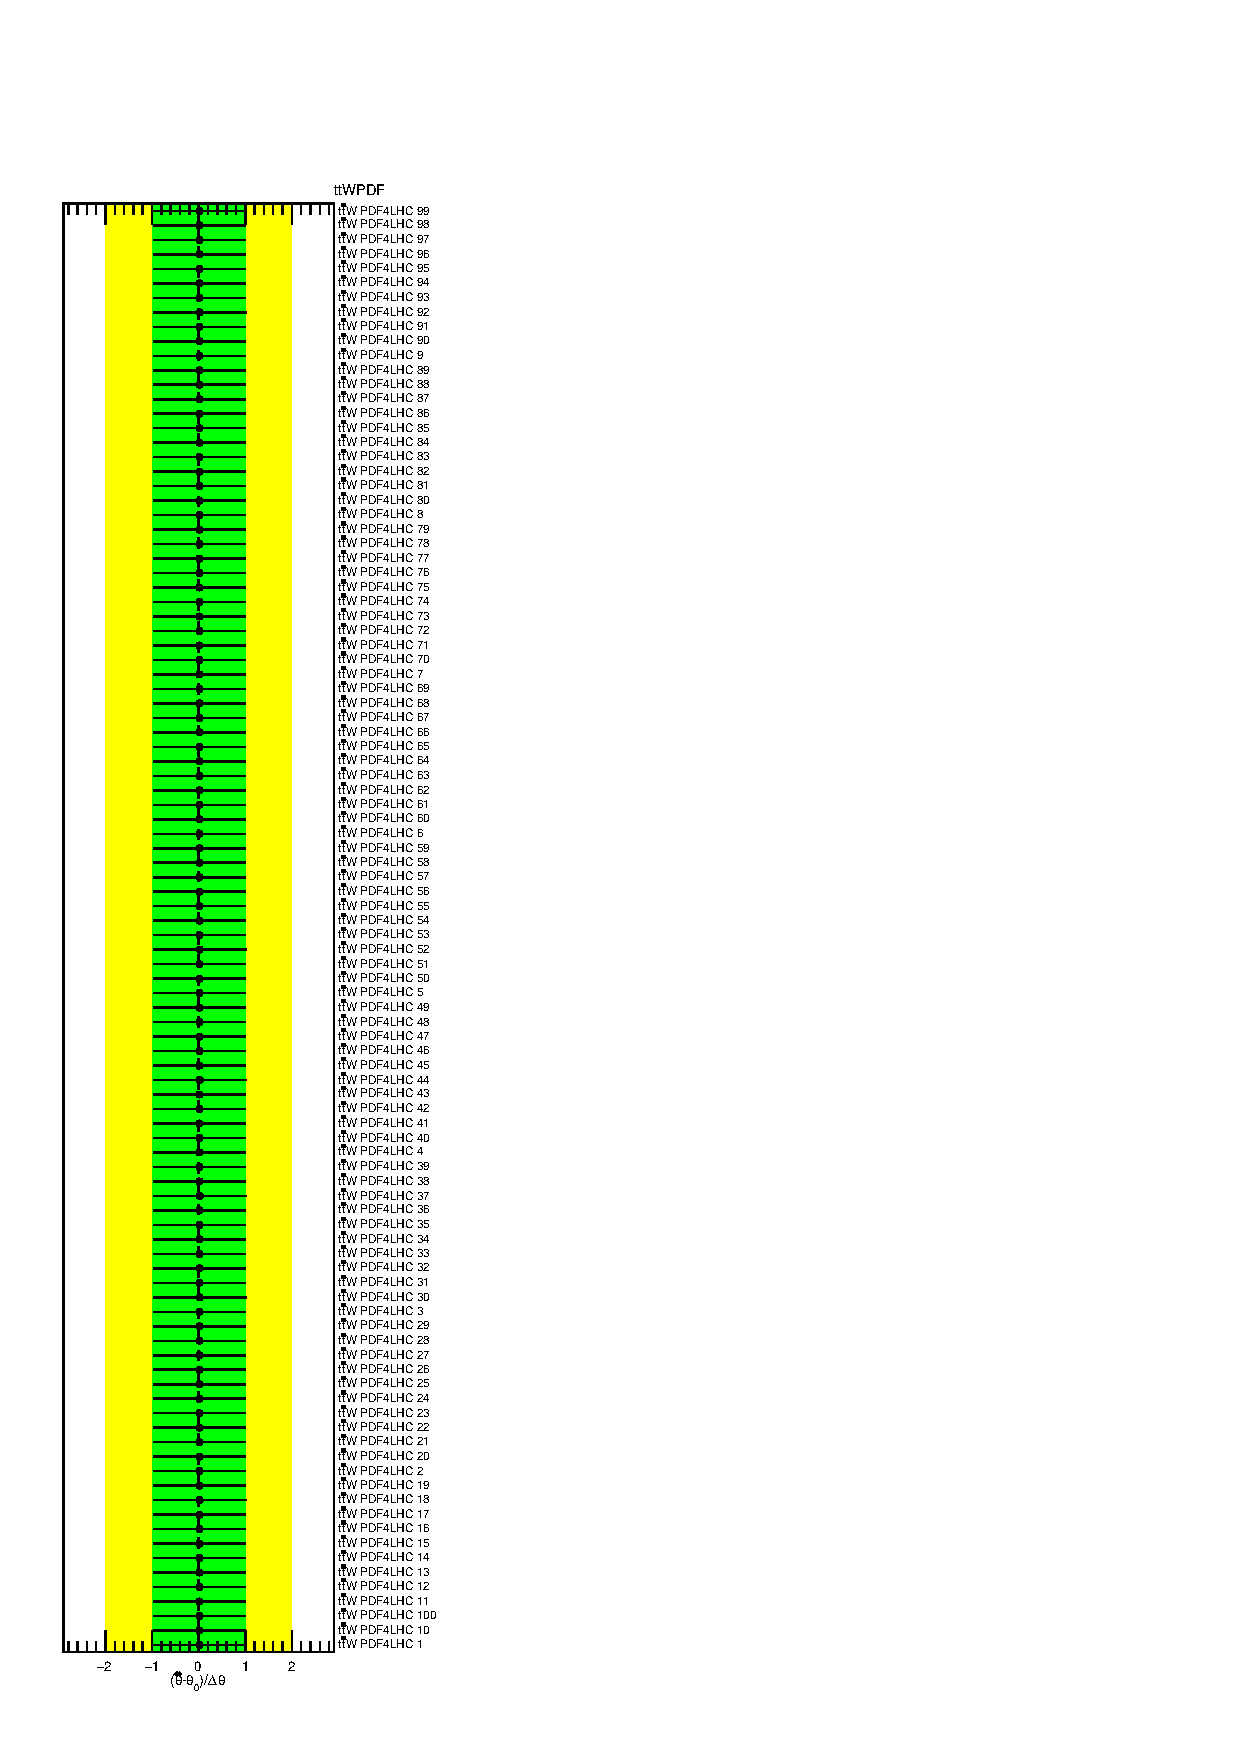
\includegraphics[height=0.9\textheight]{Chapter5_tHq/NPs/SS/SingleCR/CRBONLY_NuisPar_ttWPDF}
   \caption{Constraints and pulls on the NPs of the \tWH PDFs in the CR-only--background-only fit of the \dilepSStau channel.
   Each NP is shown as the relative change from its nominal value.
   The green and yellow areas represent the $\pm1\sigma$ and $\pm2\sigma$ deviations from the nominal value of the NP, respectively. 
   The points represent the best-fit value for the NP and the uncertainty bars represent the post-fit uncertainty.}
  \label{fig:Appendix:AdditionalResults:SS:CRBONLY:CRBONLY_NuisPar_tWHPDF}
\end{figure}

\begin{figure}[h]
  \centering
  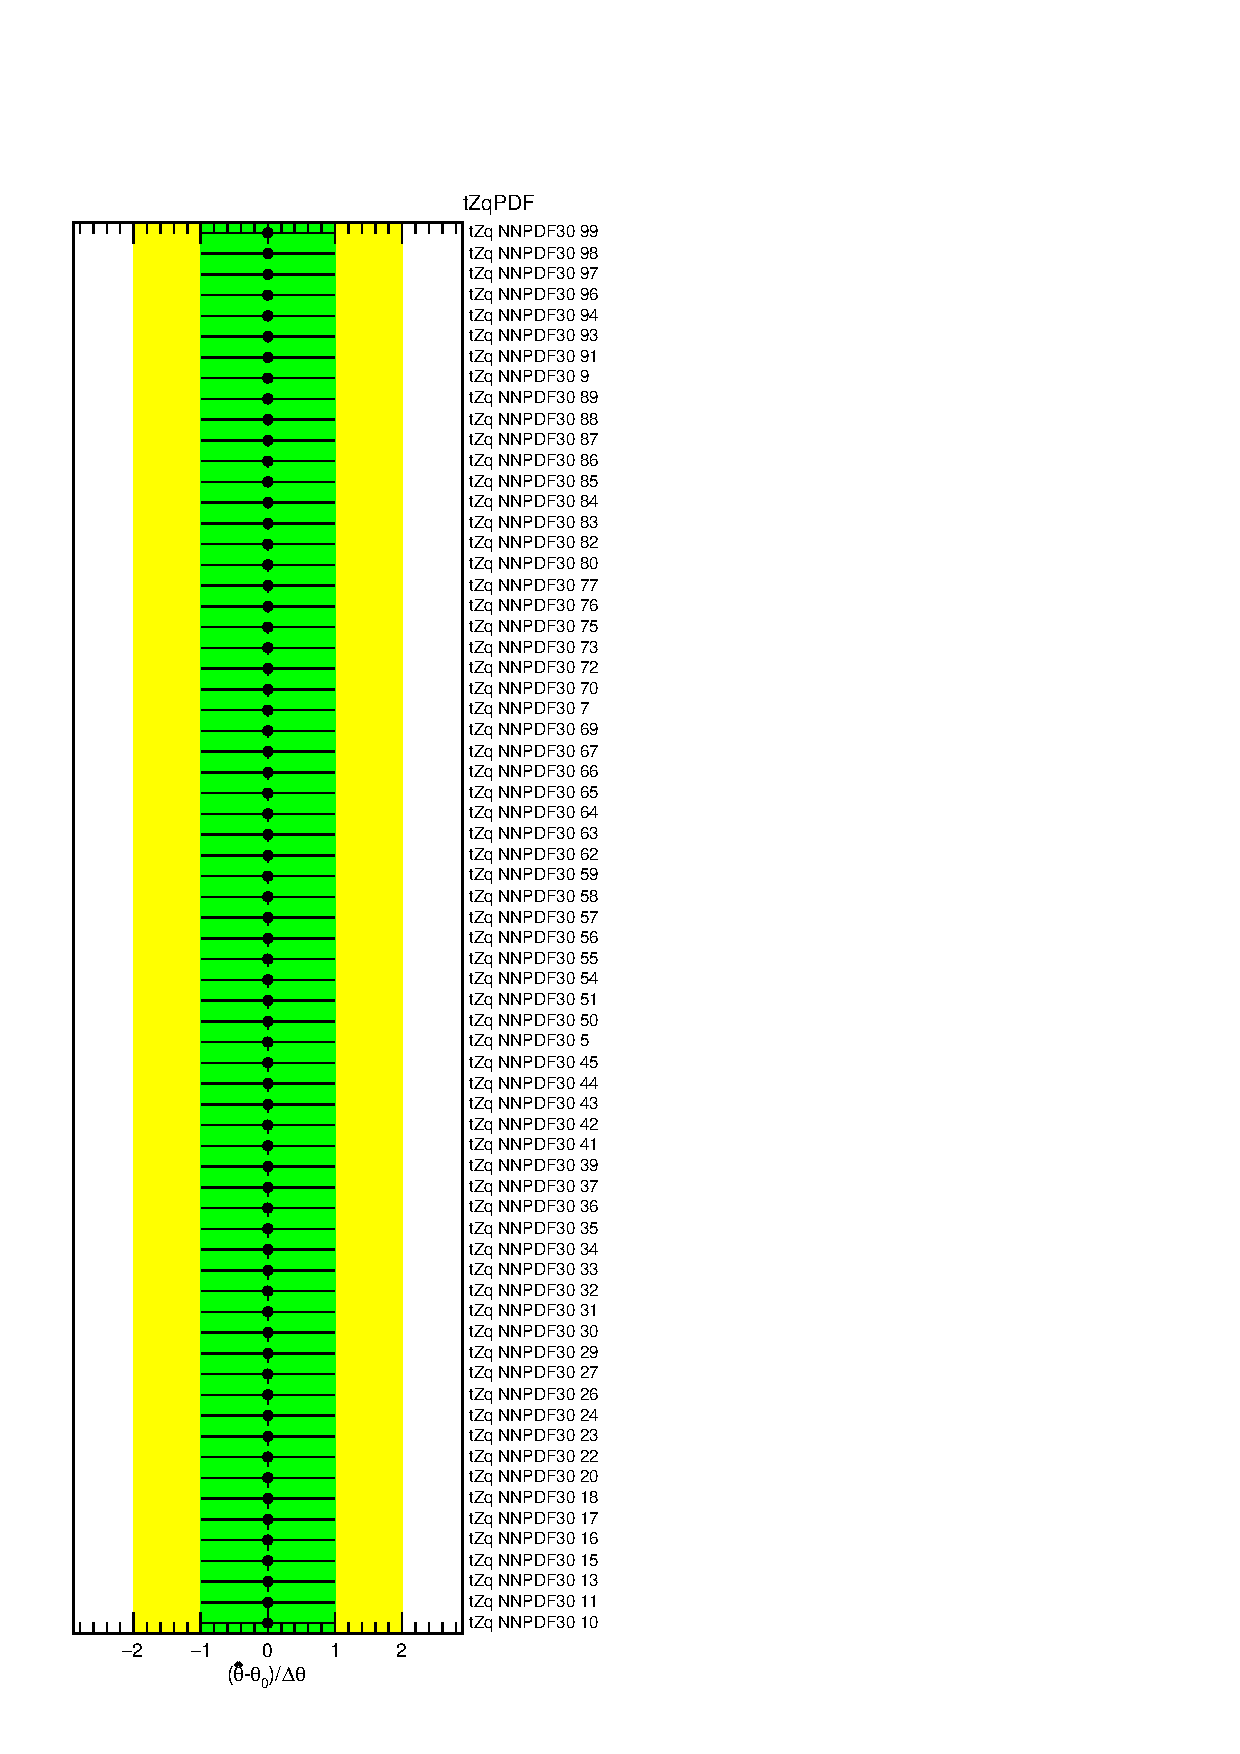
\includegraphics[width=.95\linewidth]{Chapter5_tHq/NPs/SS/SingleCR/CRBONLY_NuisPar_tZqPDF}
   \caption{Constraints and pulls on the NPs of the \tZq PDFs in the CR-only--background-only fit of the \dilepSStau channel.
   Each NP is shown as the relative change from its nominal value.
   The green and yellow areas represent the $\pm1\sigma$ and $\pm2\sigma$ deviations from the nominal value of the NP, respectively. 
   The points represent the best-fit value for the NP and the uncertainty bars represent the post-fit uncertainty.}
  \label{fig:Appendix:AdditionalResults:SS:CRBONLY:CRBONLY_NuisPar_tZqPDF}
\end{figure}

\begin{figure}[h]
  \centering
  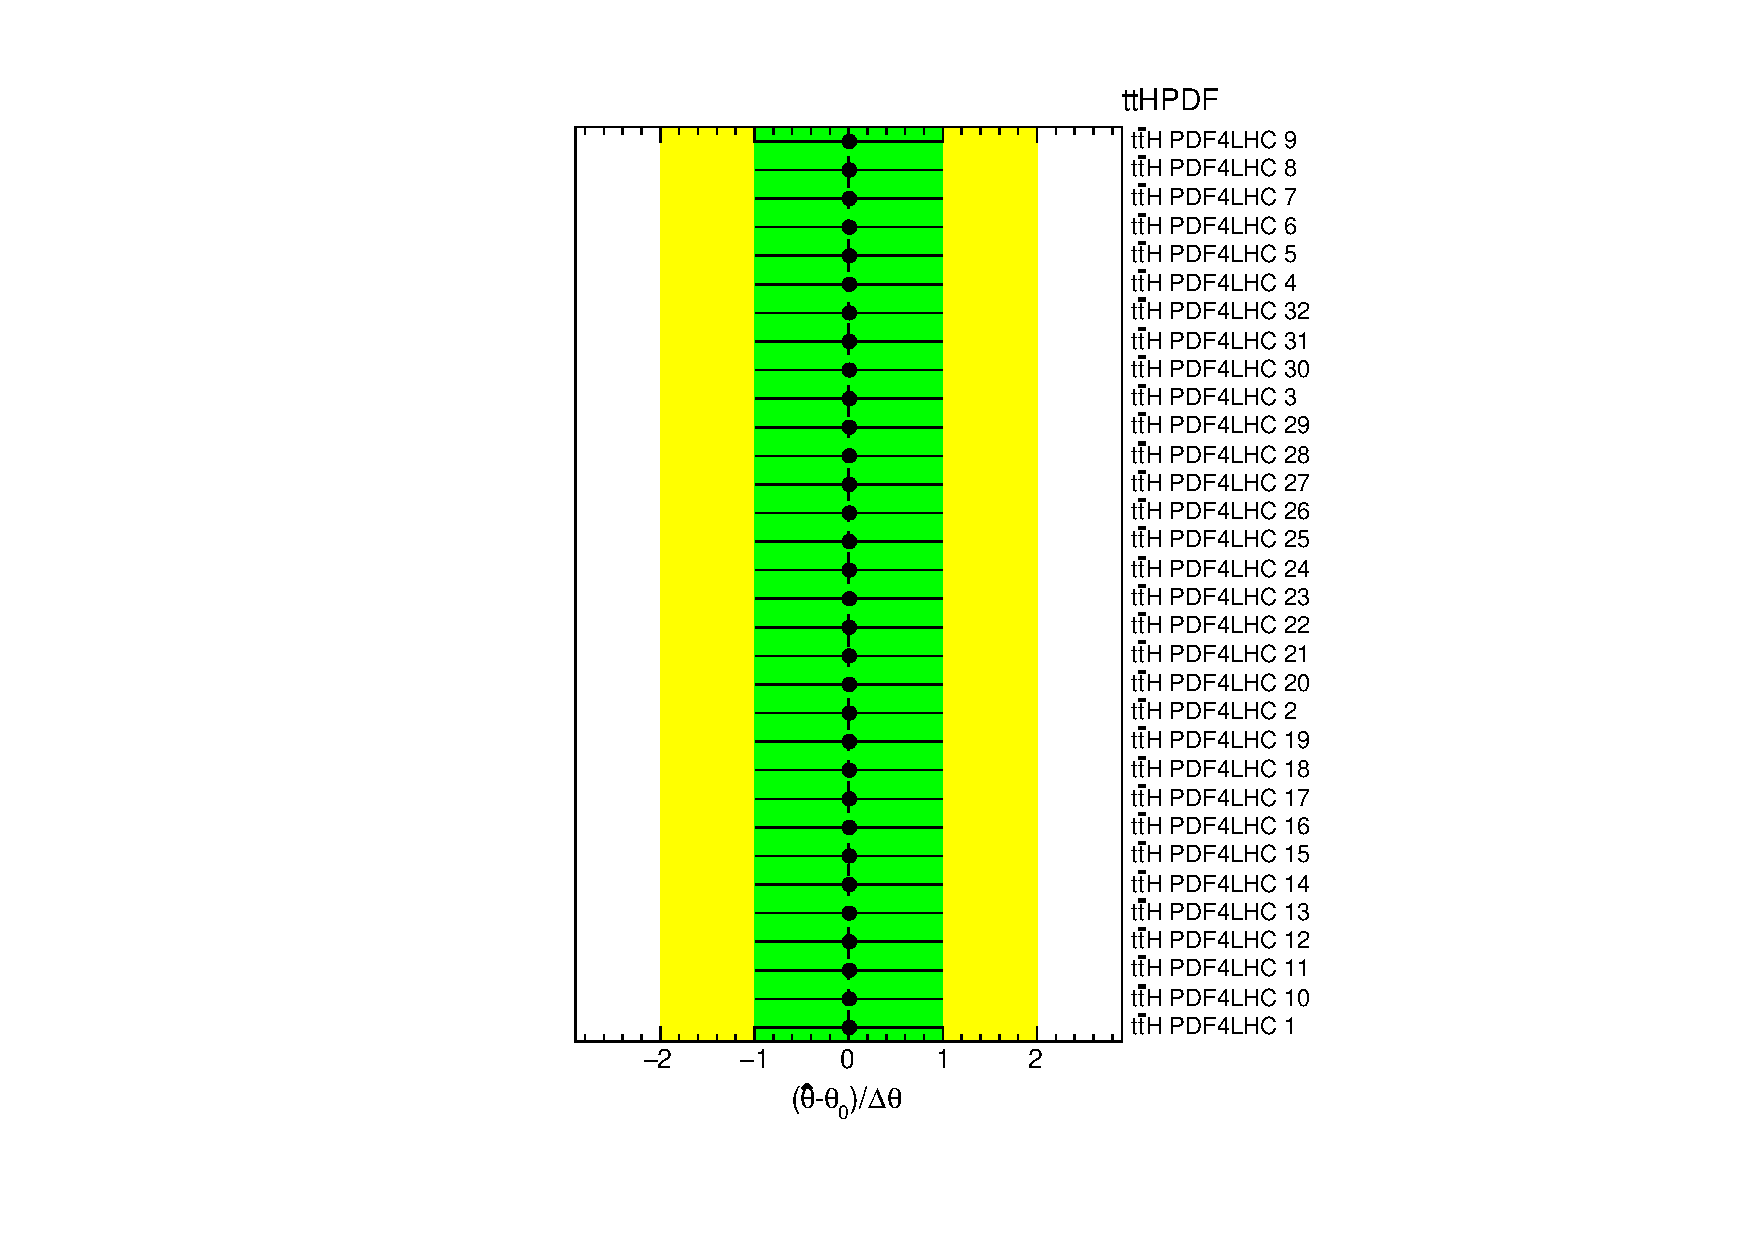
\includegraphics[width=.95\linewidth]{Chapter5_tHq/NPs/SS/SingleCR/CRBONLY_NuisPar_ttHPDF}
   \caption{Constraints and pulls on the NPs of the \ttH PDFs in the CR-only--background-only fit of the \dilepSStau channel.
   Each NP is shown as the relative change from its nominal value.
   The green and yellow areas represent the $\pm1\sigma$ and $\pm2\sigma$ deviations from the nominal value of the NP, respectively. 
   The points represent the best-fit value for the NP and the uncertainty bars represent the post-fit uncertainty.}
  \label{fig:Appendix:AdditionalResults:SS:CRBONLY:CRBONLY_NuisPar_ttHPDF}
\end{figure}

\begin{figure}[h]
  \centering
  \includegraphics[width=.95\linewidth]{Chapter5_tHq/NPs/SS/SingleCR/CRBONLY_NuisPar_ttZPDF}
   \caption{Constraints and pulls on the NPs of the \ttZ PDFs in the CR-only--background-only fit of the \dilepSStau channel.
   Each NP is shown as the relative change from its nominal value.
   The green and yellow areas represent the $\pm1\sigma$ and $\pm2\sigma$ deviations from the nominal value of the NP, respectively. 
   The points represent the best-fit value for the NP and the uncertainty bars represent the post-fit uncertainty.}
  \label{fig:Appendix:AdditionalResults:SS:CRBONLY:CRBONLY_NuisPar_ttZPDF}
\end{figure}

%\begin{figure}[h]
%  \centering
%  \includegraphics[width=.95\linewidth]{Chapter5_tHq/NPs/SS/SingleCR/CRBONLY_NuisPar_ttbarPDF}
%   \caption{Constraints and pulls on the NPs of the \ttbar PDFs in the CR-only--background-only fit of the \dilepSStau channel.}
%  \label{fig:Appendix:AdditionalResults:SS:CRBONLY:CRBONLY_NuisPar_ttbarPDF}
%\end{figure}

\begin{figure}[h]
  \centering
  \includegraphics[height=0.9\textheight]{Chapter5_tHq/NPs/SS/SingleCR/CRBONLY_NuisPar_ttWPDF}
   \caption{Constraints and pulls on the NPs of the \ttW PDFs in the CR-only--background-only fit of the \dilepSStau channel.
   Each NP is shown as the relative change from its nominal value.
   The green and yellow areas represent the $\pm1\sigma$ and $\pm2\sigma$ deviations from the nominal value of the NP, respectively. 
   The points represent the best-fit value for the NP and the uncertainty bars represent the post-fit uncertainty.}
  \label{fig:Appendix:AdditionalResults:SS:CRBONLY:CRBONLY_NuisPar_ttWPDF}
\end{figure}


\begin{figure}[h]
  \centering
  \includegraphics[height=0.9\textheight]{Chapter5_tHq/NPs/SS/SingleCR/CRBONLY_NuisPar_VVPDF}
   \caption{Constraints and pulls on the NPs of the diboson PDFs in the CR-only--background-only fit of the \dilepSStau channel.
   Each NP is shown as the relative change from its nominal value.
   The green and yellow areas represent the $\pm1\sigma$ and $\pm2\sigma$ deviations from the nominal value of the NP, respectively. 
   The points represent the best-fit value for the NP and the uncertainty bars represent the post-fit uncertainty.}
  \label{fig:Appendix:AdditionalResults:SS:CRBONLY:CRBONLY_NuisPar_VVPDF}
\end{figure}

\FloatBarrier
%%%%%%%%%%%%%%%%%%%%%%%%%%%
%           CRONLY BONLY SS  :: NormFactors          %
%%%%%%%%%%%%%%%%%%%%%%%%%%%
\subsection{Normalisation factors  in the \dilepSStau CR-only--background-only fit}
\label{sec:Appendix:AdditionalResults:SS:CRBONLY:NormFactors}

\begin{figure}[h]
\centering
\begin{subfigure}{.5\textwidth}
  \centering
  \includegraphics[width=.95\linewidth]{Chapter5_tHq/NPs/SS/SingleCR/CRBONLY_NormFactors_statOnly}
  \caption{Using only the statistical uncertainties.}
\end{subfigure}%
\begin{subfigure}{0.5\textwidth}
  \centering
  \includegraphics[width=.95\linewidth]{Chapter5_tHq/NPs/SS/SingleCR/CRBONLY_NormFactors}
  \caption{Considering all uncertainties.}
\end{subfigure}
\caption{Normalisation factors in the CR-only--background-only fit of the \dilepSStau channel.
 These results are obtained with (a) the fit considering only the statistical uncertainty and (b) the
considering all uncertainty sources.}
\label{fig:Appendix:AdditionalResults:SS:CRBONLY:NormFactors}
\end{figure}



%%%%%%%%%%%%%%%%%%
%              Full data fit SS              %
%%%%%%%%%%%%%%%%%%
\section{Full-data-unblinded fit in the \dilepSStau channel}
\label{sec:Appendix:AdditionalResults:SS:Unblinded}


%%%%%%%%%%%%%%%%%%%%%
%              Full data fit SS  :: Pulls            %
%%%%%%%%%%%%%%%%%%%%%
\subsection{Pull plots in the \dilepSStau full-data-unblinded fit}
\label{sec:Appendix:AdditionalResults:SS:Unblinded:Pulls}



%%%%%%%%%%%%%%%%%%%%%%%%%%
%              Full data fit SS  :: NormFactors            %
%%%%%%%%%%%%%%%%%%%%%%%%%
\subsection{Normalisation factors  in the \dilepSStau full-data-unblinded fit}
\label{sec:Appendix:AdditionalResults:SS:Unblinded:NormFactors}

The Figure~\ref{fig:Appendix:AdditionalResults:SS:Unblinded:NormFactors} 
represents graphically the results given in Equations~\ref{eq:ChaptH:FinalFit:SS:mu},
and \ref{eq:ChaptH:FinalFit:SS:ktt}  of Section~\ref{sec:ChaptH:Fit:FullFit:SS:results}.
Observe that the uncertainties are symmetrical. 

\begin{figure}[h]
\centering
\begin{subfigure}{.5\textwidth}
  \centering
  \includegraphics[width=.95\linewidth]{Chapter5_tHq/NPs/SS/SingleCR/Unblinded_NormFactors_statOnly}
  \caption{Using only the statistical uncertainties.}
\end{subfigure}%
\begin{subfigure}{0.5\textwidth}
  \centering
  \includegraphics[width=.95\linewidth]{Chapter5_tHq/NPs/SS/SingleCR/Unblinded_NormFactors}
  \caption{Considering all uncertainties.}
\end{subfigure}
\caption{Normalisation factors in the full-data-unblinded fit of the \dilepSStau channel.
These results are obtained with (a) the fit considering only the statistical uncertainty and (b) the
considering all uncertainty sources.}
\label{fig:Appendix:AdditionalResults:SS:Unblinded:NormFactors}
\end{figure}

\end{comment}


